% Dies ist die Hauptdatei, von der aus das Gesamtdokument erzeugt wird.  Diese
% Datei sollten Sie zunächst umbenennen, damit sie keinen generischen Namen
% hat!  Dann wird sie mit LuaLaTeX kompiliert.

% In der Datei defs.tex werden alle globalen LaTeX-spezifischen Einstellungen
% vorgenommen
% Jede LaTeX-Datei beginnt mit der Dokumentenklasse.  Für diese Vorlage wurde
% die Klasse "scrreprt" von KOMA-Script gewählt, die in etwa der
% Standardklasse "report" entspricht, allerdings wesentlich mehr Möglichkeiten
% bietet und im gewissen "moderner" ist.  Eine sehr ausführliche Dokumentation
% zu KOMA-Script findet man unter der folgenden Adresse:
% http://mirrors.ctan.org/macros/latex/contrib/koma-script/doc/scrguide.pdf
\documentclass[
  % die Schriftgröße - sollten Sie nicht ändern
  fontsize=12pt,
  % das Papierformat, also DIN A4
  paper=A4,
  % Literaturverzeichnis ins Inhaltsverzeichnis
  bibliography=totoc,
  % andere Verzeichnisse ebenfalls ins Inhaltsverzeichnis
  listof=totoc,
  % abgesetzte Formeln linksbündig
  fleqn,
  % für die Satzspiegelkonstruktion - siehe KOMA-Doku
  DIV=12,
  % Bindekorrektur (linker Rand) - evtl. anpassen
  BCOR=1mm,
  % die im Text verwendeten Sprachen (u.a. für das Paket babel); die
  % letztgenannte (!) Sprache ist die Standardsprache; "n"german steht für die
  % neue Rechtschreibung
  english,ngerman,
  % weil (s.u.) das Paket geometr verwendet wird
  usegeometry,
  % wie Absätze gesetzt werden: ohne Einzug, halbe Zeile Abstand
  parskip=half-
]{scrreprt}

% Beschriftungen für Tabellen kommen linksbündig über die Tabelle
\KOMAoption{captions}{tableheading,nooneline}
\setcaptionalignment[figure]{c}
\setcaptionalignment[table]{l}

% wird für die Titelseite benötigt
\usepackage{geometry}

% Standardpaket für Lokalisation, siehe Option "ngerman" oben
\usepackage{babel}
% Laden von optimierten Trennmustern
\babelprovide[hyphenrules=ngerman-x-latest]{ngerman}

% Standardpaket für mathematische Zusatzfunktionen; wenn Sie keine
% mathematischen Formeln brauchen, können Sie diese Zeile löschen
\usepackage{amsmath}

% die Hauptschrift Libertinus
\usepackage{libertinus-otf}
% die "Schreibmaschinenschrift" Anonymous Pro, angepasst
\usepackage{AnonymousPro}
\setmonofont{AnonymousPro}[Scale=MatchLowercase,FakeStretch=0.85]

% etwas größerer Zeilenabstand als im Buchsatz
\linespread{1.1}

% Paket für Feinkorrekturen an der Typographie, das für ein ausgewogeneres
% Schriftbild sorgt
\usepackage{microtype}

% Paket für kontextsensitive Anführungszeichen
\usepackage{csquotes}
% Shortcut, damit aus dem eigentlich falschen Zeichen " richtige
% Anführungszeichen je nach Sprache werden
\MakeOuterQuote{"}

% Paket, das den Befehl \includegraphics ermöglicht
\usepackage{graphicx}

% komfortablere Aufzählungen als in Standard-LaTeX; ein Beispiel findet man in
% chap3.tex
\usepackage{enumitem}

% Paket für mehr als die üblichen Standardfarben
\usepackage[dvipsnames]{xcolor}
% Definition der "Hausfarben" der HAW
\definecolor{haw}{HTML}{003CA0}
\definecolor{haw2}{HTML}{0096D2}
\definecolor{haw3}{HTML}{A0BEDC}
\definecolor{darkgreen}{rgb}{0, 0.5, 0}
\definecolor{background}{HTML}{EEEEEE}
\definecolor{delim}{RGB}{20,105,176}
\colorlet{punct}{red!60!black}
\colorlet{numb}{magenta!60!black}

% typographisch anspruchsvolle Tabellen; siehe chap3.tex
\usepackage{booktabs}

% zum Erstellen des Literaturverzeichnisses; der gängige Stil APA ist hier
% bereits eingestellt
\usepackage[style=apa]{biblatex}
% eine Beispieldatei für ein Literaturverzeichnis
\addbibresource{bachelorarbeit.bib}

% für die Erzeugung der Grafiken in chap3.tex; wenn Sie PGF/TikZ nicht
% verwenden wollen, können Sie diese Zeilen entfernen
\usepackage{tikz}
% Zusatzbibliotheken für TikZ, die in den genannten Beispielen verwendet
% werden
\usetikzlibrary{calc,intersections,angles,3d}

% für die Erzeugung des Codeblocks in chap3.tex; wenn in Ihrer Arbeit keine
% Codeblöcke vorkommen, können Sie diese Zeilen entfernen
\usepackage{listings}

% see https://tex.stackexchange.com/questions/83085/how-to-improve-listings-display-of-json-files
\lstdefinelanguage{json}{
    basicstyle=\normalfont\ttfamily,
    numbers=left,
    numberstyle=\scriptsize,
    stepnumber=1,
    numbersep=8pt,
    showstringspaces=false,
    breaklines=true,
    frame=lines,
    backgroundcolor=\color{background},
    literate=
    *{0}{{{\color{numb}0}}}{1}
        {1}{{{\color{numb}1}}}{1}
        {2}{{{\color{numb}2}}}{1}
        {3}{{{\color{numb}3}}}{1}
        {4}{{{\color{numb}4}}}{1}
        {5}{{{\color{numb}5}}}{1}
        {6}{{{\color{numb}6}}}{1}
        {7}{{{\color{numb}7}}}{1}
        {8}{{{\color{numb}8}}}{1}
        {9}{{{\color{numb}9}}}{1}
        {:}{{{\color{punct}{:}}}}{1}
        {,}{{{\color{punct}{,}}}}{1}
        {\{}{{{\color{delim}{\{}}}}{1}
        {\}}{{{\color{delim}{\}}}}}{1}
        {[}{{{\color{delim}{[}}}}{1}
        {]}{{{\color{delim}{]}}}}{1},
}
% see https://tex.stackexchange.com/questions/152829/how-can-i-highlight-yaml-code-in-a-pretty-way-with-listings
\newcommand\YAMLcolonstyle{\color{red}\mdseries}
\newcommand\YAMLkeystyle{\color{black}\bfseries}
\newcommand\YAMLvaluestyle{\color{blue}\mdseries}

\makeatletter

\newcommand\language@yaml{yaml}

\expandafter\expandafter\expandafter\lstdefinelanguage
\expandafter{\language@yaml}
{
    keywords={true,false,null,y,n},
    keywordstyle=\color{darkgray}\bfseries,
    basicstyle=\YAMLkeystyle,
    sensitive=false,
    comment=[l]{\#},
    morecomment=[s]{/*}{*/},
    commentstyle=\color{purple}\ttfamily,
    stringstyle=\YAMLvaluestyle\ttfamily,
    moredelim=[l][\color{orange}]{\&},
    moredelim=[l][\color{magenta}]{*},
    moredelim=**[il][\YAMLcolonstyle{:}\YAMLvaluestyle]{:},
    morestring=[b]',
    morestring=[b]",
    literate =    {---}{{\ProcessThreeDashes}}3
        {>}{{\textcolor{red}\textgreater}}1
        {|}{{\textcolor{red}\textbar}}1
        {\ -\ }{{\mdseries\ -\ }}3,
}

\lst@AddToHook{EveryLine}{\ifx\lst@language\language@yaml\YAMLkeystyle\fi}
\makeatother
\newcommand\ProcessThreeDashes{\llap{\color{cyan}\mdseries-{-}-}}

\lstdefinelanguage{math}{
    keywords={SIGNED, UNSIGNED},
    sensitive=true,
    morekeywords={bis},
    keywordstyle=\color{blue}\bfseries,
    comment=[l]\%,
    string=[b]",
    morestring=[b]',
    moredelim=*[s][\color{gray}]{/*}{*/},
    morekeywords={[2]Beispiel},
    keywordstyle={[2]\color{haw2}\bfseries},
}

% Anpassung des Erscheinungsbildes des Codeblocks; mehr dazu in der
% Dokumentation des Pakets "listings"
\lstdefinestyle{mystyle}{
    backgroundcolor=\color{gray!20},
    keywordstyle=\color{haw2},
    numberstyle=\footnotesize\color{haw},
    basicstyle=\ttfamily\small,
    captionpos=t,
    frame=single,
    framerule=0pt,
    keepspaces=true,
    numbers=left,
    numbersep=6pt,
    belowcaptionskip=1em,
    aboveskip=\bigskipamount,
}

\lstdefinestyle{custom_daniel}{
    backgroundcolor=\color{gray!20},
    basicstyle=\ttfamily\small,
    keywordstyle=\color{haw2},
    commentstyle=\color{gray},
    numberstyle=\footnotesize\color{haw},
    stringstyle=\color{darkgreen},
    numbers=left,
    breaklines=true,
    keepspaces=true,
    showspaces=false,
    showstringspaces=false,
}
\lstset{style=mystyle}
% damit es "Codeblock" und nicht "Listing" heißt
\renewcommand{\lstlistingname}{Codeblock}

% für die Verlinkung innerhalb des PDF-Dokuments, für PDF-Lesezeichen und
% PDF-Metadaten; dieses Paket sollte üblicherweise immer als letztes geladen
% werden
\usepackage[colorlinks=true,allcolors=haw,hyperfootnotes=false,pageanchor=true,linktoc=all]{hyperref}

% für die Druckversion können Sie die obige Zeile durch die folgende ersetzen,
% damit Links nicht blau dargestellt werden:
% \usepackage[draft]{hyperref}

% Metadaten des PDF-Dokumentes; setzen Sie hier Ihren eigenen Namen sowie den
% Titel Ihrer Arbeit ein
\hypersetup{pdfauthor={Daniel Freire Mendes}}
\hypersetup{pdftitle={Performance-Optimierung von Datenbanken}}

\usepackage{subcaption}
\usepackage{float}
\usepackage[labelfont=bf]{caption}
% \includeonly{benchmarks}
% BibTex see here: https://github.com/Hannah-Sten/TeXiFy-IDEA/issues/1390
% Wenn das Kommentarzeichen entfernt wird, kann man mit einem Befehl wie
%
% \includeonly{chap2,chap3}
%
% erreichen, dass nur ausgewählte Dateien kompiliert werden.  Das ist für die
% Arbeit an umfangreichen Dokumenten hilfreich, weil es Zeit spart.  Für das
% Erstellen des fertigen Dokuments muss der Befehl natürlich wieder
% auskommentiert werden, damit alle Referenzen aktuell sind und die
% Seitenzahlen stimmen.

% Hier beginnt das eigentliche Dokument.  Sie können weitere Dateien
% hinzufügen und natürlich auch vorhandene weglassen.  Die vorhandene
% Dateistruktur ist lediglich als Beispiel gedacht.
\begin{document}
% In dieser Umgebung wird die Titelseite separat vom restlichen Text gesetzt
\begin{titlepage}
  % andere Seitenränder als im Rest der Arbeit
  \newgeometry{lmargin=2cm,tmargin=7mm,rmargin=5mm,bmargin=1cm}
  % die "Hausfarbe" der HAW; diese und die folgenden Einstellungen sind lokal
  % und gelten nur innerhalb der Umgebung "titlepage"
  \color{haw}
  % Blocksatz für die Titelseite deaktivieren
  \raggedright
  % Logo rechtsbündig setzen
  \hfill
\includegraphics[width=7cm]{PNGs/General/HAW_Marke_RGB_300dpi}\\

  % vertikaler Abstand
  \vspace{5cm}

  % Wahl der "Hausschrift" Open Sans der HAW, die als Schrift auf Ihrem
  % Rechner installiert sein muss
  \setmainfont{Open Sans}
  % etwas kleiner als üblich
  \small
  % fett und in Majuskeln
  \textbf{BACHELORARBEIT}

  % vertikaler Abstand
  \vspace{8mm}

  % der Titel der Arbeit als "Seite in der Seite"; natürlich müssen Sie hier
  % Ihren Titel eintragen
  \begin{minipage}{0.8\linewidth}
    % Wahle der zweiten "Hausschrift" der HAW, die ebenfalls auf Ihrem Rechner
    % bereits vorhanden sein muss
    \setmainfont{Martel Heavy}
    % ziemlich große Schrift
    \LARGE
    % [1mm] steht jeweils für einen etwas größeren Durchschuss
    Performance -\\[1mm]
    Optimierung\\[1mm]
    von Datenbanken\\
    % am Ende noch ein waagerechter Strich, das CD will es so...
    \,\rule{11mm}{1.2mm}
  \end{minipage}

  % vertikaler Abstand, überraschenderweise
  \vspace{1cm}

  % hier korrektes Datum und Ihren Namen eingeben
  % TODO(Daniel): update this
  vorgelegt am 26. März 2022\\
  Daniel Freire Mendes

  % letzter vertikaler Abstand für heute
  \vspace{5cm}

  % noch eine "Seite in der Seite", etwas nach rechts geschoben
  \hspace*{37mm}
  \begin{minipage}{0.5\linewidth}
    % Namen und Titel der beiden Prüfer eintragen
    \begin{tabular}{@{}ll}
      Erstprüferin: & Prof. Dr. Stefan Sarstedt\\[-.3mm]
      Zweitprüfer: & Prof. Dr. Olaf Zukunft \\
    \end{tabular}\\

    % noch ein horizontaler Strich
    \,\rule{9mm}{1mm}\\[1.5mm]

    \textbf{HOCHSCHULE FÜR ANGEWANDTE}\\
    \textbf{WISSENSCHAFTEN HAMBURG}\\
    Department Informatik\\
    Berliner Tor 7\\
    20099 Hamburg
  \end{minipage}
\end{titlepage}
% setzt die Geometrie wieder auf die Standardwerte zurück
\restoregeometry

% für die Seite mit dem Abstract keine Seitenzahl ausgeben
\thispagestyle{empty}
% TODO(Daniel): write text here
\section*{Zusammenfassung}

% Hier ersetzen Sie bitte die vorhandenen Texte durch Ihre eigenen
% Zusammenfassungen
Der Arbeit beginnt mit einer kurzen Beschreibung ihrer zentralen Inhalte, in
der die Thematik und die wesentlichen Resultate skizziert werden.  Diese
Beschreibung muss sowohl in deutscher als auch in englischer Sprache vorliegen
und sollte eine Länge von etwa 150 bis 250 Wörtern haben.  Beide Versionen
zusammen sollten nicht mehr als eine Seite umfassen.  Die Zusammenfassung
dient u.\,a.\ der inhaltlichen Verortung im Bibliothekskatalog.

% Zum Wechseln der Sprache siehe den Kommentar in chap3.tex
{
  \begin{otherlanguage}{english}
    % TODO(Daniel): write text here
    \section*{Abstract}

    The thesis begins with a brief summary of its main contents, outlining the
    subject matter and the essential findings.  This summary must be provided
    in German and in English and should range from 150 to 250 words in length.
    Both versions combined should not comprise more than one page.  Among
    other things, the abstract is used for library classification.
  \end{otherlanguage}
}

% In der Titelei werden römische Ziffern für die Seitenzahlen verwendet;
% gleichzeitig wird durch diesen Befehl die aktuelle Seitenzahl auf eins
% gesetzt
\pagenumbering{Roman}

% Inhaltsverzeichnis
\tableofcontents

% Abbildungsverzeichnis, kann evtl. weggelassen werden
\listoffigures

% Tabellenverzeichnis, kann evtl. weggelassen werden
\listoftables

% weitere Verzeichnisse (z.B. Codeblöcke) sind theoretisch möglich

% neue Seite, vorsichtshalber
\clearpage
% ab jetzt arabische Ziffern und wieder auf eins setzen
\pagenumbering{arabic}
%! Author = danielmendes
%! Date = 21.10.24
\chapter{Überblick}

\section{Einführung in Benchmarks}

Benchmarks dienen dazu, praktisch und effektiv zu untersuchen, wie sich ein
System unter Last verhält. Die wichtigste Erkenntnis, die man aus Benchmarks
gewinnen kann, sind die Probleme und Fehler, die man systematisch dokumentieren
und nach Priorität abarbeiten sollte. Das Ziel von Benchmarks ist die Reduzierung
und Bewertung von unerwünschtem Verhalten sowie die Analyse, wie sich das
System derzeit und unter simulierten, zukünftigen, anspruchsvolleren Bedingungen
verhalten könnte.

Es gibt zwei verschiedene Techniken für Benchmarks. Die erste zielt darauf ab,
die Applikation als Ganzes zu testen (full-stack). Dabei wird nicht nur die
Datenbank getestet, sondern die gesamte Applikation, einschließlich des Webservers,
des Netzwerks und des Applikationscodes. Der Ansatz dahinter ist, dass ein Nutzer
genauso lange auf eine Abfrage warten muss, wie das gesamte System benötigt.
Daher sollte diese Wartezeit so gering wie möglich sein. Es kann dabei vorkommen,
dass MySQL nicht immer das Bottleneck ist.\footnote{Gemeint ist ein Engpass beim Transport von Daten oder Waren, der maßgeblichen Einfluss auf die Abarbeitungsgeschwindigkeit hat. Optimierungsversuche an anderer Stelle führen oft nur zu geringen oder gar keinen messbaren Verbesserungen der Gesamtsituation. (\cite{bottleneck})}

Full-Stack-Benchmarks haben jedoch auch Nachteile. Sie sind schwieriger zu erstellen
und insbesondere schwieriger korrekt einzurichten. Wenn man lediglich verschiedene
Schemas und Abfragen in MySQL auf ihre Performance testen möchte, gibt es sogenannte
Single-Component-Benchmarks. Diese analysieren ein spezifisches Problem in der
Applikation und sind deutlich einfacher zu erstellen. Ein weiterer Vorteil besteht
darin, dass nur ein Teil des gesamten Systems getestet wird, wodurch die Antwortzeiten
kürzer sind und man schneller Ergebnisse erhält.

Wenn bei Benchmarks schlechte Designentscheidungen getroffen werden, kann dies zu einer
falschen Interpretation des Systems führen, da die Ergebnisse nicht die Realität widerspiegeln.
Die Größe des Datensatzes und des Workloads muss realistisch sein. Idealerweise verwendet
man einen Snapshot\footnote{Snapshots bestehen größtenteils aus Metadaten, die den Zustand Ihrer Daten definieren, und sind keine vollständige Duplikation der Daten auf Ihrer Festplatte. Snapshots werden häufig für Test-/Entwicklungsaufgaben verwendet. (\cite{snapshot}) } des tatsächlichen produktiven Datensatzes.
Gibt es keine Produktionsdaten, sollten die Daten und der Workload simuliert werden,
da realistische Benchmarks komplex und zeitaufwendig sein können.

Häufige Fehler beim Durchführen von Benchmarks sind unter anderem, dass nur ein kleiner Teil
der tatsächlichen Datensatzgröße verwendet wird und die Datensätze unkorrekt gleichmäßig
verteilt sind. In der Realität können Hotspots auftreten. Bei zufällig generierten Werten
kommt es hingegen häufig zu unrealistisch gleichmäßig verteilten Datensätzen. Ein weiterer
Fehler besteht darin, dass man beim Testen einer Anwendung nicht das tatsächliche
Benutzerverhalten nachstellt. Wenn gleiche Abfragen in einer Schleife ausgeführt werden,
muss man außerdem auf das Caching achten, da sonst falsche Annahmen über die Performance
getroffen werden können. Zudem wird oft die Warmmachphase des Systems vollständig ignoriert.
Kurze Benchmarks können schnell zu falschen Annahmen über die Performance des Systems führen.

Um verlässliche Ergebnisse zu erhalten, sollte ein Benchmark ausreichend lange laufen,
um den stabilen Zustand des Systems zu beobachten, insbesondere bei Servern mit großen
Datenmengen und viel Speicher. Dabei ist es wichtig, so viele Informationen wie möglich zu
erfassen und sicherzustellen, dass der Benchmark wiederholbar ist, da unzureichende oder
fehlerhafte Tests wertlos sind. Außerdem ist es wichtig, die Ergebnisse in einem Diagramm
darzustellen, da auftretende Phänomene sonst anhand einer tabellarischen Darstellung nicht
erkannt werden können.


\section{Measures}
\begin{itemize}[label={--}]
    \item \textbf{Durchsatz (Throughput):} Der Durchsatz ist die Anzahl an Transaktionen pro Zeiteinheit.
    Er ist standardisiert, und Datenbankanbieter versuchen, diesen zu optimieren.
    Meistens werden Transaktionen pro Sekunde (oder manchmal pro Minute) als Einheit verwendet.
    \item \textbf{Antwortzeiten (Latenz):} Die Antwortzeit misst die gesamte Zeit, die für eine Abfrage benötigt wird.
    Diese kann, abhängig von der Applikation, in Mikrosekunden (µs), Millisekunden (ms), Sekunden oder Minuten angegeben werden.
    Von dieser Zeit können aggregierte Antwortzeiten wie Durchschnitt, Maximum, Minimum und Perzentile abgeleitet werden.
    Das Maximum ist oft eine weniger sinnvolle Metrik, da es sich nicht gut wiederholen lässt.
    Daher nutzt man eher Perzentile bei den Antwortzeiten.
    Wenn beispielsweise das 95. Perzentil der Antwortzeit bei 5 ms liegt, bedeutet dies, dass mit einer Wahrscheinlichkeit von 95 \% die Abfrage in weniger als 5 ms abgeschlossen ist.
    \item \textbf{Nebenläufigkeit (Concurrency):} Die Nebenläufigkeit auf dem Webserver lässt sich nicht zwangsläufig auf den Datenbankserver übertragen.
    Eine genauere Messung der Gleichzeitigkeit auf dem Webserver besteht darin, zu bestimmen, wie viele gleichzeitige Anfragen zu einem bestimmten Zeitpunkt ausgeführt werden.
    Es kann auch geprüft werden, ob der Durchsatz sinkt oder die Antwortzeiten steigen, wenn die Gleichzeitigkeit zunimmt.
    Beispielsweise benötigt eine Website mit „50.000 Benutzern gleichzeitig“ vielleicht nur 10 oder 15 gleichzeitig laufende Abfragen.
    \item \textbf{Skalierbarkeit (Scalability):} Skalierbarkeit ist wichtig für Systeme, die ihre Performance unter unterschiedlich starken Workloads beibehalten müssen.
    Ein ideales System würde doppelt so viele Abfragen beantworten (Throughput), wenn doppelt so viele „Arbeiter“ versuchen, die Aufgaben zu erfüllen.
    Die meisten Systeme sind jedoch nicht linear skalierbar und zeigen Leistungseinbußen, wenn die Parameter variieren.
\end{itemize}


\section{Tools}\label{sec:tools}

\subsection{Einführung}\label{subsec:einfuhrung}

Als Haupttool, um Benchmarktests durchzuführen, habe ich mich für Sysbench \cite{sysbench_repo}
entschieden. Sysbench ist ein Open-Source-Tool, das ein skriptfähiges, multi-threaded Benchmark-Tool
ist, das auf LuaJIT basiert. Es wird auch hauptsächlich für Datenbankbenchmarks verwendet, kann
jedoch auch dazu eingesetzt werden, beliebig komplexe Arbeitslasten zu erstellen, die keinen
Datenbankserver erfordern. Dabei werden Tests auf verschiedenen Systemressourcen, wie CPU, S
peicher, I/O und Datenbanken wie MySQL \cite{sysbench_mysql} verwendet.

Im Zuge der Recherchearbeit habe ich mir auch andere Benchmarking-Tools betrachtet, wie z.B.
Benchbase \cite{DifallahPCC13} oder mybench \cite{mybench_repo}. Die größten Vorteile von
Sysbench habe ich in der Skriptfähigkeit und Flexibilität gesehen. D.h. dass ich benutzerdefinierte
Benchmarks schneller und unkompliziert erstellen kann. Außerdem hat sich Sysbench als de facto
Standard im Bereich der Datenbankbenchmarks etabliert \cite{mybench_comparison}. Dadurch stehen
eine breite Nutzerbasis und viele verfügbare Ressourcen zur Verfügung. Im Vergleich zu den
anderen Tools bietet allerdings Sysbench eine weniger präzise Steuerung der Ergebnisrate
und der Transaktionen. Außerdem haben Tools wie mybench die Möglichkeit, in Echtzeit umfassende
Visualisierungen darzustellen. Damit können Metriken live in einem Diagramm angezeigt werden
\cite{mybench_user_interface}. Dieses Feature ist sicherlich hilfreich, aber in meinem Fall habe
ich abgewogen und bin zu dem Entschluss gekommen, dass die einfachere Bedienung für mich der
ausschlaggebende Grund, neben dem Fakt, dass Sysbench der de facto Standard ist.

Trotzdem kann man nicht komplett auf Graphen verzichten, da beispielweise Entwicklungen
im Laufe einer Zeitmessung in einem Kurvenverlauf deutlich besser zu erkennen sind als in einer CSV-Datei.
Anhand der reinen Zahlen aus diesen Tabellen fallen diese wiederkehrende Trends unter anderem nicht direkt auf.
Die Kennzahlen, die mithilfe von Sysbench ermittelt werden, werden in einer CSV-Datei gespeichert.
Um diese tabellarische Form in eine Grafische umzuwandeln, gibt es unterschiedliche Tools, die widerum
eigene Vor- und Nachteile bieten.

Die erste mögliche Alternative stellt das Tool Gnuplot \cite{gnuplot} dar.
Mit diesem lassen sich CSV-Dateien sehr gut darstellen. Wenn man aber beispielweise nur bestimmte Spalten
aus der Tabelle anzeigen lassen will, dann kommt man schnell an seine Granzen.
Um besser Anpassungsfähig sein zu können, habe ich mich letztlich dazu entschieden ein eigenes Python-Script
zu schreiben, die mithilfe der Libraries pandas (//TODO (Daniel): find source) matplotlib.pyplot (//TODO (Daniel): find source)
die Graphen erstellt.

\subsection{Einführung in die Tools}\label{subsec:einfuhrung-in-die-tools}

Als allererstes muss der MySQL-Server (oder eine anderes relationales Datenbankverwaltungssystem, das von Sysbench
unterstützt wird) lokal auf dem Rechner gestartet sein. Wichtig ist dabei die User -und Passwortdaten zu merken, da
diese von den Sysbench - Benchmarks benötigt werden. Nachdem das RDBMS gestartet worden ist, muss zudem eine
Datenbank erstellt werden. Dies könnte unter anderem so aussehen:

\begin{lstlisting}[label={lst:create database}]
CREATE DATABASE sbtest;
\end{lstlisting}

Nachdem man die Datenbank erstellt hat, muss das Tool Sysbench zunächst installiert werden.
Als nächstes machen wir uns mit dem Tool und den verschiedenen Argumenten,
die beim Aufruf mitübergeben werden müssen oder können, vertraut.
Hier ist eine Auflistung mit den übergebenen Argumenten:

\begin{itemize}
    \item \texttt{--db-driver}: Gibt den Treiber für die Datenbank an, die Sysbench verwenden soll. In diesem Fall \texttt{mysql}, um MySQL-Datenbanken zu testen.
    \item \texttt{--mysql-host}: Der Hostname oder die IP-Adresse des MySQL-Servers. Standardmäßig wird \texttt{localhost} verwendet, wenn nichts angegeben wird.
    \item \texttt{--mysql-user}: Der Benutzername, mit dem Sysbench auf die MySQL-Datenbank zugreift.
    \item \texttt{--mysql-password}: Das Passwort für den MySQL-Benutzer. Falls der Benutzer kein Passwort hat oder der Zugriff über eine andere Authentifizierungsmethode erfolgt, kann dieses Argument weggelassen werden.
    \item \texttt{--mysql-db}: Der Name der MySQL-Datenbank, auf die zugegriffen wird. In diesem Beispiel \texttt{sbtest}.
    \item \texttt{--time}: Gibt die Laufzeit des Benchmarks in Sekunden an und muss immer mit angegeben werden.
    \item \texttt{--report-interval}: Gibt das Intervall in Sekunden an, in dem Zwischenergebnisse während des Tests ausgegeben werden.
    Sofern \texttt{--report-interval} nicht gesetzt wird, werden die Ergebnisse erst am Ende des Tests angezeigt.
    \item \texttt{--tables}: Die Anzahl der Tabellen, die für den Test erstellt werden sollen. Standardmäßig wird nur eine Tabelle erstellt.
    \item \texttt{--table-size}: Die Anzahl der Datensätze (Zeilen) pro Tabelle. Muss auch nicht zwingend angegebend werden.
\end{itemize}

Neben den sieben aufgelisteten Argumenten gibt es zwei weitere wichtige Optionen:
\begin{enumerate}
    \item Wie im Abschnitt~\ref{einfuhrung} erwähnt, kann ein Lua-Skript angegeben werden, um eigene
    Tabellen zu erstellen, Beispieldaten einzufügen und bestimmte Abfragen durchzuführen.
    Dazu muss am Ende der Sysbench-Befehlszeile lediglich der Pfad zur Lua-Datei hinzugefügt werden.
    Ein erklärendes Beispiel dazu folgt weiter unten in diesem Abschnitt.
    \item Die Methode, den Sysbench ausführen soll, muss ebenfalls spezifiziert werden.
    Auch dieser wird am Ende der Sysbench-Befehlszeile angehängt.
\end{enumerate}

Zunächst schauen wir ein kurzes Demo-Beispiel, denn es gibt die Möglichkeit die Datenbank
auf Performance zu testen, ohne selbst eigene SQL-Befehle zu schreiben. Dafür gibt es vordefinierte Testtypen von Sysbench.
Auf diese Weise kann man schnell die Korrektheit der Einrichtung des Tools überprüfen, bevor man Lua-Scripts
für die eigenen Bedürfnisse schreibt.

Man kann unter anderen zwischen diesen Testtypen wählen:
\begin{itemize}
    \item \textbf{oltp\_insert}: Prüft die Fähigkeit der Datenbank, Daten schnell und effizient einzufügen und
    simuliert eine Umgebung, in der viele Schreiboperationen ausgeführt werden.
    \item \textbf{oltp\_read\_only}: Fokussiert sich auf die Performance bei Leseoperationen und
    eignet sich, um die Leistung bei einer rein lesenden Arbeitslast zu testen.
    \item \textbf{oltp\_read\_write}: Simuliert eine realistische Arbeitslast, bei der sowohl Lese- als
    auch Schreiboperationen gleichzeitig durchgeführt werden.
\end{itemize}

Des Weiteren gibt es auch unterschiedliche Methoden, die mit den Testtypen kombiniert werden können.

\begin{itemize}
    \item \item \textbf{prepare}: Bereitet die Datenbank für den Test vor, u.a. das Einfügen von benötigten Datensätze.
    \item \textbf{run}: Ist die Ausführungsphase des Tests. Je nach Testtyp führt diese Methode die spezifizierten Operationen aus,
    wie etwa das Einfügen von Daten (oltp\_insert), das Abfragen von Daten (oltp\_read\_only) oder beides (oltp\_read\_only).
    Dabei wird die Performance der Datenbank unter der angegebenen Arbeitslast gemessen.
    \item \textbf{cleanup}: Diese Methode sorgt dafür, dass nach Abschluss des Tests alle Testdaten entfernt werden.
    Sie stellt die Datenbank in ihren ursprünglichen Zustand zurück und stellt sicher,
    dass keine Testdaten zurückbleiben, die eine mögliche produktive Umgebung beeinträchtigen könnten.
\end{itemize}

Für das Demo-Beispiel wählen wir den Testtypen \textbf{oltp\_read\_write} und allen Methoden aus.
Für die Methode run würde unsere Query so aussehen, wobei \texttt{YOUR\_USER} und \texttt{YOUR\_PASSWORD}
entsprechend ersetzt werden müssten:

\begin{lstlisting}[style=custom_daniel,label={lst:sysbenchrun}]
sysbench oltp_read_write \
  --db-driver=mysql \
  --mysql-user=YOUR_USER \
  --mysql-password=YOUR_PASSWORD \
  --mysql-db="sbtest" \
  --time=10 \
  --report-interval=1 \
  run
\end{lstlisting}

Wenn man nur diese Query ausführt, fällt er auf, dass die Query scheitert. Deshalb bietet es sich an ein Shell-Script
zu schreiben, indem zuerst \texttt{prepare} aufgerufen wird und als Nächstes erst \texttt{run}. Die Ergebnisse der Log-Datei
speichert man sich dann in einer Datei und aus dieser Datei erstellt man eine CSV-Datei, mit der man später die Graphen
erstellen lässt. Und als letzten Schritt ruft man die \texttt{cleanup}-Methode auf, damit bei erneuter Ausführung keine
Fehler entstehen, bzw. die Produktivumgebung nicht gestört wird, wenn diese sonst beeinflusst werden würde.

Dies ist das Shell-Script, dass zuständig ist für den kompletten Ablauf:
\lstinputlisting[
    language=bash,
    caption=Sysbench Script,
    label={lst:sysbench_monitor},
    style=custom_daniel,
]{Scripts/Demo/sysbench_monitor.sh}

\lstinputlisting[
    language=gnuplot,
    caption=Gnuplot Script,
    label={lst:plot_sysbench},
    style=custom_daniel,
]{Scripts/Demo/plot_sysbench.gp}

Das Python-Script, das zuständig ist für die Graphgenerierung muss als Argument zum einen
die CSV-Datei übermittelt bekommen und zum anderen kann es nur eine bestimmte Auswahl an
Messwerten übergeben, damit nur für diese die Graphen erzeugt werden.
Dies ist das zuständige Python-Script:

\lstinputlisting[
    language=python,
    caption=Pandas Graph Generator,
    label={lst:pandas_plot},
    style=custom_daniel,
]{Scripts/Join_Type/generateplot.py}

% missing: how the script and results exactly are fpr Join_Type and explain the measures underneath


\begin{figure}[!ht]
    \centering
    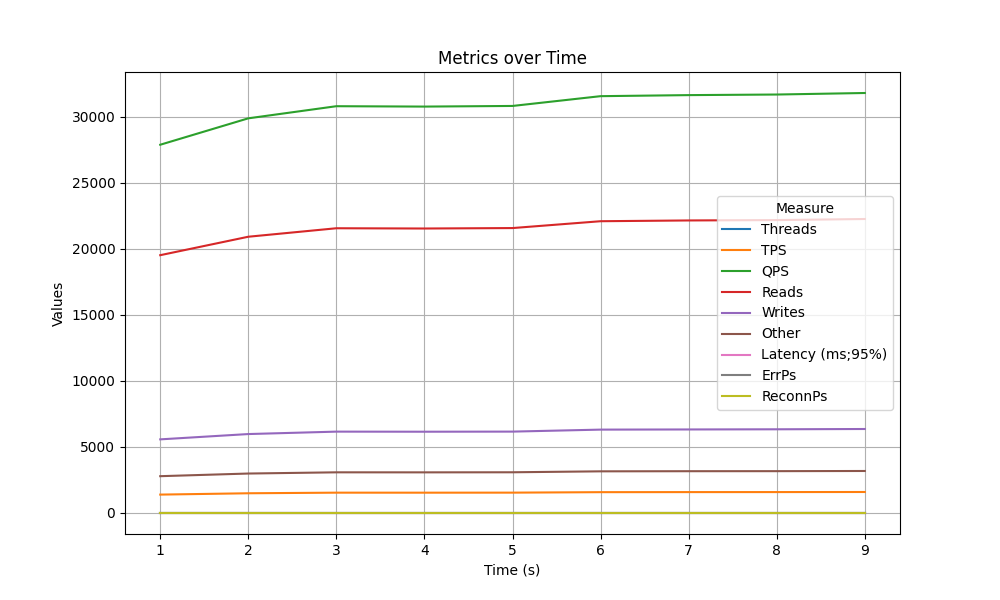
\includegraphics[width=.8\textwidth]{PNGs/Demo/Summary}
    \caption[Pandas - Beispiel]{Grafik generiert mithilfe des Pythontools Pandas}
    \label{demo-pandas}
\end{figure}

\begin{figure}[!ht]
    \centering
    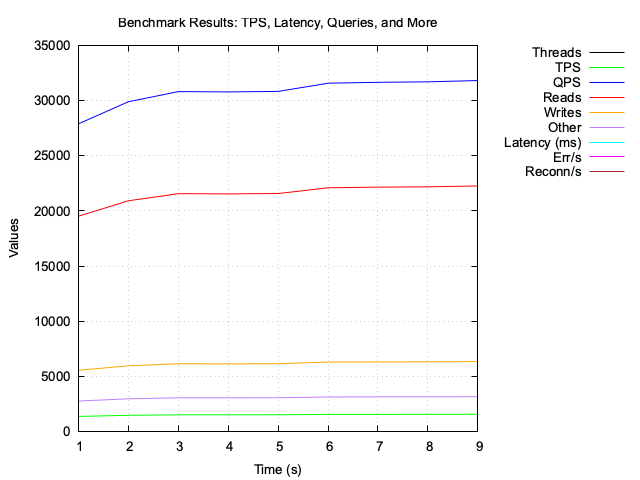
\includegraphics[width=.8\textwidth]{PNGs/Demo/sysbench_output}
    \caption[Gnuplot - Beispiel]{Grafik generiert mithilfe von Gnuplot}
    \label{demo-gnuplot}
\end{figure}


\begin{itemize}
    \item \textbf{Threads}: Die Anzahl der gleichzeitig verwendeten Threads.
    Mehr Threads können die Parallelität erhöhen, jedoch kann eine zu hohe Anzahl
    die Leistung beeinträchtigen, wenn das System überlastet wird.
    \item \textbf{TPS (Transactions Per Second)}: Die Anzahl der Transaktionen pro Sekunde.
    Ein höherer Wert deutet auf eine bessere Datenbankleistung hin.
    \item \textbf{QPS (Queries Per Second)}: Die Anzahl der Abfragen pro Sekunde.
    Ein höherer Wert ist besser und zeigt die Effizienz bei der Verarbeitung von Abfragen.
    \item \textbf{Reads}: Die Anzahl der Leseoperationen.
    Mehr Leseoperationen sind im Allgemeinen besser, da sie eine höhere Datenauslastung anzeigen, was jedoch auch vom spezifischen Anwendungsfall abhängt.
    \item \textbf{Writes}: Die Anzahl der Schreiboperationen.
    Ähnlich wie bei den Leseoperationen: Mehr Schreibvorgänge sind besser, solange die Performance erhalten bleibt.
    \item \textbf{Other}: Bezieht sich auf andere Arten von Operationen, die weder als Reads noch als Writes kategorisiert werden.
    Ein höherer Wert ist gut, solange er nicht zu einer Überlastung führt.
    \item \textbf{Latency (ms; 95\%)}: Die durchschnittliche Zeit in Millisekunden, die benötigt wird, um Anfragen zu bearbeiten, wobei der Wert im 95. Perzentil betrachtet wird.
    Niedrigere Werte sind besser, da sie auf schnellere Reaktionszeiten hinweisen.
    \item \textbf{ErrPs (Errors Per Second)}: Die Anzahl der Fehler pro Sekunde.
    Ein niedriger Wert ist wünschenswert, da er auf eine höhere Stabilität und Zuverlässigkeit des Systems hinweist.
    \item \textbf{ReconnPs (Reconnects Per Second)}: Die Anzahl der Wiederverbindungen pro Sekunde.
    Ein niedrigerer Wert ist ebenfalls besser, da häufige Wiederverbindungen auf Stabilitätsprobleme hindeuten können.
\end{itemize}

%! Author = danielmendes
%! Date = 11.12.24
\chapter{Projektdurchführung}\label{ch:projektdurchfuhrung}

\section{GitHub Action}\label{sec:github-action}

Im Laufe der Bachelorarbeit sind immer mehr unterschiedliche Projekte dazugekommen, die alle das Orchestrator-Skript benutzen.
Dadurch sind immer mehr Fallunterscheidungen in diesem Skript erforderlich geworden, und man hat schnell den Überblick verloren, wenn man Änderungen vorgenommen hat.
Um zu überprüfen, ob diese Änderungen negative Nebeneffekte haben, mussten jedes Mal alle Skripte nacheinander ausgeführt werden, was nicht nur zeitintensiv war, sondern auch hohe Lasten für den lokalen Rechner bedeutete.
Eine Möglichkeit wäre es gewesen, die Skripte parallel durchlaufen zu lassen, um Zeit zu sparen, aber damit wäre das Lastenproblem nicht gelöst worden.
Eine deutlich bessere Variante ist die Auslagerung in eine Pipeline.
In meinem Fall habe ich mich für GitHub Actions entschieden.
Vereinfacht gesagt sollen in der GitHub Action alle Skripte parallel ausgeführt und am Ende alle Output-Dateien in einen Ordner zusammen als GitHub Artifact hochgeladen werden.
Anschließend kann man die Zip-Datei herunterladen und überprüfen, ob alle Ergebnisse noch mit der Erwartung übereinstimmen.
Wenn fehlerhafte Änderungen hochgeladen wurden, scheitert der Workflow-Run direkt, und man hat einen guten Überblick über alle Projekte.

Damit dies funktioniert, muss eine YAML-Datei im Ordner \texttt{.github/workflows/} erstellt werden.
Anschließend bekommt der Workflow einen Namen und man kann definieren, wann er getriggert werden soll.
In meinem Fall, wenn sich etwas im \texttt{./github}-Ordner verändert, im \texttt{Projects/}-Ordner, in dem sich alle Lua-Skripte befinden, oder wenn sich das Orchestrator-Skript und die in diesem Skript benutzten Python-Dateien ändern.
Als Nächstes muss man eine JSON-Datei mit den Informationen zu den exportierten Variablen und den verwendeten Skripten befüllen und den einzelnen Projekten einen Namen geben.
Diesen Namen muss man auch in der Matrix definieren, damit die Informationen parallel aus der JSON-Datei entnommen und die Befehle ausgeführt werden können.

\lstinputlisting[
    language=Json,
    caption=JSON mit Konfiguration der Script,
    label={lst:script_configuration},
    style=custom_daniel,
    basicstyle=\ttfamily\scriptsize,
]{Scripts/Join_Type/11_Pattern.json}

Anschließend muss man wie schon bei den Skripts davor die Umgebungsvariablen in der YAML – Datei definieren, wenn es sich um vertrauliche Informationen handeln sollte, bietet es sich an GitHub Secrets zu benutzen.
Danach beginnen erst die eigentlichen Schritte, die in dem Workflow ausgeführt werden.
Zunächst muss man das Repository auschecken und die passende Konfiguration aus der JSON – Datei laden, die dem Testtypen entspricht aus der Matrix.
Anschließend muss man nur noch die Abhängigkeiten installieren.
Da immer die gleichen Dependencies geladen werden, kann man auch GitHub Cache benutzen und einmal die installierten Dependencies als Cache hochladen und anschließend nur noch den Cache herunterladen.
Danach muss man den MySQL - Container mit den korrekten Umgebungsvariablen starten und dann kann auch schon die das Orchestrator - Skript ausgeführt werden.
Um das Ganze aufzuräumen, kann man dem MySQL Container wieder stoppen und als letzten Schritt muss man noch den Output Ordner als Artifact hochladen.

\lstinputlisting[
    language=yaml,
    caption=Ausschnitt aus der Workflow - Datei,
    label={lst:workflow_yaml},
    style=custom_daniel,
]{Scripts/Join_Type/12_Workflow.yaml}

\textbf{TODO: Optimierungen, die man Durchführen kann:}
\newline Tried these here:
\begin{itemize}
    \item GitHub Artifacts
    \item GitHub Cache $\rightarrow$ deprecated after 7 days and only works
    \item (GitHub Repo) or dedicated feature branch $\rightarrow$ give GitHub action write permission so push is allowed
    \item (Google Cloud Storage (GCS), AWS S3 or Azure Storage)
\end{itemize}
%! Author = danielmendes
%! Date = 29.11.24

\chapter{Indizes}\label{ch:indexes}

Das folgende Kapitel befasst sich mit der Indexierung und den damit verbundenen Performance-Optimierungen, die näher erläutert werden.
Zunächst werden einige Grundlagen der Indexierung betrachtet.
Anschließend werden die verschiedenen Arten von Indizes näher erläutert und unterschiedliche Benchmarks mit ihnen durchgeführt.
Im letzten Schritt werden die Ergebnisse analysiert, um festzustellen, welche Verwendung der Indizes am besten funktioniert.

\section{Grundlagen}\label{sec:indexing-grundlagen}

Indizes sind Datenstrukturen, die von Speicher-Engines (engl.\ storage engines) verwendet werden, um unter anderem Zeilen schneller zu finden (\cite[S. 147--189]{schwartz2012high}).
Die Storage-Engine ist eine Kernkomponente eines Datenbankmanagementsystems, die für die Speicherung und Verwaltung der Daten verantwortlich ist.
Verschiedene Storage-Engines unterscheiden sich hinsichtlich ihrer Indexfunktionalität sowie der Unterstützung von Transaktionen und Sperrmechanismen.
Im weiteren Verlauf werden verschiedene Indextypen vorgestellt, die nicht von allen Engines unterstützt werden.

Die Indizes haben einen großen Einfluss auf die Datenbank-Performance und werden mit zunehmender Größe der Datenbank immer wichtiger, da das Scannen aller Tupel zunehmend aufwendiger wird.
Weniger ausgelastete Datenbanken können ohne ordnungsgemäße Indizes gut funktionieren, aber die Leistung kann rapide sinken, wenn die Datenmenge wächst.
Wenn ein solches Problem auftritt, ist die Index-Optimierung oft der effektivste Weg, um die Abfrageleistung schnell zu verbessern.
Um wirklich optimale Indizes zu erstellen, ist es häufig notwendig, Abfragen umzuschreiben.
Besonders nützlich sind Indizes bei Abfragen, die Joins zwischen mehreren Tabellen enthalten, da sie ermöglichen, die Anzahl der zu prüfenden Tupel erheblich zu reduzieren, wenn eine einschränkende Bedingung vorliegt.
Wie genau Indizes erstellt werden müssen, wird im Laufe dieses Kapitels geklärt.


Um die Funktionsweise eines Indexes anschaulicher zu erklären, wird als Beispiel ein wissenschaftliches Fachbuch betrachtet.
Am Ende dieser Bücher gibt es meist ein Stichwortverzeichnis oder Register.
Dieses Register besteht aus einer alphabetisch geordneten Liste von Begriffen, Themen und Stichworten.
Möchte man einen Begriff nachschlagen, sucht man ihn im Stichwortverzeichnis und erhält die Seitenzahlen, auf denen er vorkommt.
In DBMS verwendet die Storage-Engine Indizes auf eine ähnliche Weise.
Sie durchsucht die Datenstruktur des Indexes nach einem Wert.
Und wenn ein Treffer gefunden wird, kann die Engine die Zeilen ermitteln, die den Treffer enthalten.
Das folgendes Beispiel veranschaulicht dies:

\begin{lstlisting}[language=SQL]
SELECT NAME FROM KUNDEN WHERE KUNDEN_ID = 7;
\end{lstlisting}

Angenommen, es existiert ein Index auf der Spalte \texttt{KUNDEN\_ID}, dann wird MySQL diesen verwenden, um Zeilen zu finden, bei denen die \texttt{KUNDEN\_ID} den Wert 7 hat.
Mit anderen Worten wird eine Suche innerhalb der Indexwerte durchgeführt und alle entsprechenden Zeilen werden zurückgegeben.

Ein Index kann Werte aus einer oder mehreren Spalten einer Tabelle enthalten.
Bei mehreren Spalten ist die Reihenfolge der Spalten im Index entscheidend, da MySQL nur effizient auf ein linkes Präfix des Indexes zugreifen kann.
Gibt man nur das zweite Attribut an, ohne das erste zu referenzieren, kann der Index nicht direkt verwendet werden.
Außerdem darf man nicht verwechseln, dass ein Index über zwei Spalten nicht gleichbedeutend ist mit zwei separaten einspaltigen Indizes.
Es gibt verschiedene Typen von Indizes, die jeweils für unterschiedliche Zwecke optimiert sind und in den nächsten Abschnitten behandelt werden.

Um zu verstehen, wie man Indizes für eine Datenbank auswählt, ist es wichtig zu wissen, welcher Teil der Abfrage am meisten Zeit in Anspruch nimmt (\cite[S. 350--353]{garcia2008database}).
Das Datenbanksystem ist so aufgebaut, dass die Tupel einer Relation üblicherweise auf viele Seiten einer Festplatte verteilt sind, die jeweils mehrere Tausend Bytes umfassen und viele Tupel speichern.
Um die Werte eines Tupels zu prüfen, muss die gesamte Seite, auch Block genannt, in den Hauptspeicher geladen werden.
Dabei kostet es kaum mehr Zeit, alle Tupel einer Seite anstatt nur ein einzelnes zu prüfen.

In der Regel stellt der Schlüssel den sinnvollsten Index für eine Tabelle dar, weshalb MySQL standardmäßig den B-Tree-Index für Primary Keys verwendet (\cite{mysql_primary_key}).
Die Entscheidung, ob für ein bestimmtes Attribut ein Index definiert werden soll, hängt von drei Faktoren ab:
Erstens ist ein Index besonders nützlich, wenn Abfragen häufig auf ein bestimmtes Attribut zugreifen.
Zweitens kann ein Index sinnvoll sein, wenn es nur wenige Tupel für einen bestimmten Wert des Attributs gibt, da dies den Festplattenzugriff bei einer Abfrage reduziert.
Sobald nicht alle Blöcke geladen werden müssen, kann der Index Zeit sparen.
Der letzte Fall betrifft Situation, in denen Tupel nach einem Attribut geclustert sind.
Durch einen Index können müssen hier weniger Datenblöcke geladenen werden, da die Werte des Attributs aufeinanderfolgender gespeichert sind.
Mit diesen Faktoren kann begründet werden, warum die Schlüssel einer Tabelle gut geeignet sind.
Zum einen kommen sie oft in Abfragen vor (erster Punkt) und zum anderen enthalten sie keine doppelten Werte, da jedes Tupel einen eindeutigen Wert hat (zweiter Punkt).

Das Auswählen von Indizes erfordert von den Entwicklern eine Tradeoff abzuwägen.
Es gibt dabei zwei Faktoren, die die Entscheidung beeinflussen.
Zum einen kann ein Index auf einem Attribut Abfragen mit diesem Attribut erheblich beschleunigen.
Zum anderen erschwert jeder Index Einfügungen, Löschungen und Aktualisierungen, da diese mehr Zeit und Aufwand erfordern.
Aber selbst wenn Modifikationen die häufigste Form von Datenbankaktionen sind, kann ein Index auf ein häufig verwendetes Attribut die Leistung verbessern.
Dies liegt daran, dass einige Modifikationsbefehle zuvor die Datenbank abfragen.
Im Kapitel \nameref{ch:partitions} wird uns dieses Thema wieder begegnen.

Um Zeitersparnis durch die Nutzung von Tupeln ohne vollständige Durchsuchung der Relation zu erreichen, müssen Indizes auf der Festplatte gespeichert werden.
Dies führt jedoch zu zusätzlichen Festplattenzugriffen.
Allgemein lässt sich sagen, dass Modifikationen in etwa doppelt so kostenintensiv sind wie der Zugriff auf den Index oder die Daten während einer Abfrage.
Damit berechnet werden kann, ob sich ein Index für eine Spalte lohnt, muss bekannt sein, mit welcher Wahrscheinlichkeit Abfragen und Modifikationen durchgeführt werden.

Um die Vorgehensweise anhand einer beispielhaften Berechnung durchzuführen, wird die folgende Tabelle benutzt (abgeändertes Beispiel aus~\cite[S. 355--357]{garcia2008database}):
\vspace{-4pt}
\begin{lstlisting}
Fakten(Id, Bestelldatum, Artikel_Id, Kunden_Id, ...)
\end{lstlisting}
\vspace{-8pt}

Der Schlüssel der Faktentabelle ist die Spalte \texttt{Id} und für die Attribute \texttt{Artikel\_Id} sowie \texttt{Kunden\_Id} wird jeweils ein Index erstellt.
Damit stehen uns insgesamt drei unterschiedliche Indexe zur Verfügung, einschließlich des Primärschlüssels.
Als Nächstes werden Befehle benötigt, bei denen die Indexe benutzt werden (siehe~\ref{lst:indexing:fakten-select-insert-queries}).
In der ersten Zeile wird nur der Kundenindex verwendet, in der zweiten nur der Artikelindex und in der Letzten fügen wie eine Zeile ein.

\vspace{-12pt}
\begin{lstlisting}[language=SQL,caption=Select-Queries für die Faktentabelle,label={lst:indexing:fakten-select-insert-queries}]
SELECT Bestelldatum, Artikel_Id FROM Fakten WHERE Kunden_Id = k;
SELECT Bestelldatum, Kunden_Id FROM Fakten WHERE Artikel_Id = a;
INSERT INTO Fakten VALUES(i, b, a, k);
\end{lstlisting}
\vspace{-8pt}

Damit berechnet werden kann, ob es sinnvoll ist, die Indizes zu erstellen, müssen bestimmte Voraussetzungen festgelegt werden.
Zuallererst wird davon ausgegangen, dass die Faktentabelle 10 Datenblöcke belegt und im Durchschnitt jeder Kunde 3 Artikel kauft, während ein Artikel von 3 Kunden gekauft wird.
Die Tupel für einen bestimmten Kunden oder Artikel sind gleichmäßig über die 10 Seiten verteilt.
Trotzdem sind mit einem Index nur 3 Festplattenzugriffe erforderlich, um die durchschnittlich 3 Tupel für einen Kunden oder Artikel zu finden.
Dazu ist ein Festplattenzugriff erforderlich, um die Seite des Indexes zu lesen und ein weiterer, um die modifizierte Seite zurückzuschreiben, falls eine Indexseite geändert werden muss.
Ohne Index sind 10 Festplattenzugriffe zum Lesen und zwei Festplattenzugriffe zum Schreiben erforderlich.
Unter diesen Bedingungen ergibt sich die folgende Kostentabelle:

\vspace{-18pt}
\begin{table}[H]
    \centering
    \setlength{\arrayrulewidth}{0.4mm}
    \[
        \begin{array}{r|c c c c}
            \textbf{Aktion} & \textbf{Kein Index} & \textbf{Kunden Index} & \textbf{Artikel Index} & \textbf{Beide Indizes} \\ \hline
            Q_1 & 10 & 4 & 10 & 4 \\
            Q_2 & 10 & 10 & 4 & 4 \\
            I   & 2  & 4  & 4  & 6 \\ \hline
            \textbf{Durchschnitt} & 2 + 8p_1 + 8p_2 & 4 + 6p_2 & 4 + 6p_1 & 6-2p_1-2p_2 \\
        \end{array}
    \]
    \vspace{-5pt}
    \caption[Performance-Vergleich]{Kosten der unterschiedlichen Queries in Abhängigkeit der Indizes}
    \label{tab:performance-queries}
\end{table}
\vspace{-25pt}

Die letzte Zeile aus Tabelle~\ref{tab:performance-queries} gibt die durchschnittlichen Kosten einer Aktion an.
Unter der Annahme, dass der Anteil der Zeit, in der die erste Abfrage ausgeführt wird, p1 beträgt und der Anteil der Zeit für die zweite Abfrage p2 ist, ergibt sich der Anteil der Zeit, in der I ausgeführt wird, zu 1 – p1 – p2.
Der Durchschnitt für den Kundenindex wird wie folgt berechnet:
\[
    4p_{1} + 10p_{2} + 4 \cdot (1 - p_{1} - p_{2}) = 4p_{1} + 10p_{2} + 4 - 4p_{1} - 4p_{2} = 4 + 6p_{2}
\]

Abhängig von den Werten für p1 und p2 kann jede der vier Optionen die geringsten Kosten für die drei Operationen verursachen.
Zum Beispiel, wenn p1 = p2 = 0,1, dann ist der Ausdruck 2 + 8p1 + 8p2 am kleinsten, sodass keine Indizes bevorzugt werden würden.
Wenn jedoch p1 = 0,5 und p2 = 0,1 gelten, ergibt ein Index für die Kunden den besten Durchschnittswert.

Damit wurde gezeigt, dass es sinnvoll ist, keinen Index zu verwenden, wenn überwiegend Einfügungen durchgeführt werden und nur sehr wenige Abfragen anfallen.
Intuitiv gilt, dass bei vielen Abfragen und einer ungefähr gleichen Häufigkeit von Abfragen, die Artikel und Kunden angeben, beide Indizes vorteilhaft sind.
Wird hingegen nur ein Typ von Abfrage häufig genutzt, sollte nur der Index definiert werden, der bei dieser Abfrageart hilft.

Es gibt zahlreiche Tools, die entwickelt wurden, um die Verantwortung der Wahl der Indizes vom Datenbankdesigner zu übernehmen.
Dabei optimiert das System sich selbst oder dem Designer werden zumindest Empfehlungen für sinnvolle Entscheidungen gegeben.
Ein bewährter Ansatz zur Auswahl von Indizes ist das sogenannte Greedy-Verfahren (\cite[S. 824]{garcia2008database}), bei dem zunächst ohne ausgewählte Indizes der Nutzen jedes Kandidaten-Index bewertet wird.
Wenn es einen Index mit positivem Nutzen gibt, wird dieser ausgewählt und anschließend wird eine Neubewertung ausgeführt, wobei davon ausgegangen wird, dass der zuvor ausgewählte Index bereits verfügbar ist.
Dieser Prozess wird so lange wiederholt, bis es keinen Kandidaten-Index mit positivem Nutzen mehr gibt.

\newpage
\section{B-Baum-Index}\label{sec:indexing-b-baum-index}

Der erste zu betrachtende Indextyp ist der B-Baum-Index (engl.\ B-Tree Index), der auf einer speziellen Baum-Datenstruktur basiert.
Diese Struktur wird von den meisten MySQL-Storage-Engines unterstützt.
Die Implementierung und Nutzung des B-Baum-Indexes kann jedoch je nach verwendeter Storage-Engine variieren.

Das Grundprinzip eines B-Baums ist, dass alle Werte in einer bestimmten Reihenfolge gespeichert werden und jede Blattseite den gleichen Abstand zum Wurzelknoten hat.

\begin{quote}
    \enquote{The height of a B+ tree depends on the number of data entries and the size of index entries.} (\cite[S. 358]{ramakrishnan2002database})
\end{quote}

Ein B-Baum-Index beschleunigt den Datenzugriff, da die Storage-Engine nicht die gesamte Tabelle durchsuchen muss, um die gewünschten Daten zu finden.
Stattdessen beginnt die Suche beim Wurzelknoten.
Die Slots im Wurzelknoten enthalten Zeiger auf Kindknoten und die Storage-Engine folgt diesen Zeigern.
Der richtige Zeiger wird durch Vergleich der Werte in den Knoten-Seiten (engl.\ node pages) ermittelt, die die oberen und unteren Grenzen der Werte in den Kindknoten definieren.
Letztlich stellt die Storage-Engine fest, ob der gewünschte Wert existiert oder ob sie erfolgreich eine Blatt (engl.\ leaf page) erreicht.

\vspace{-8pt}
\begin{figure}[H]
    \centering
    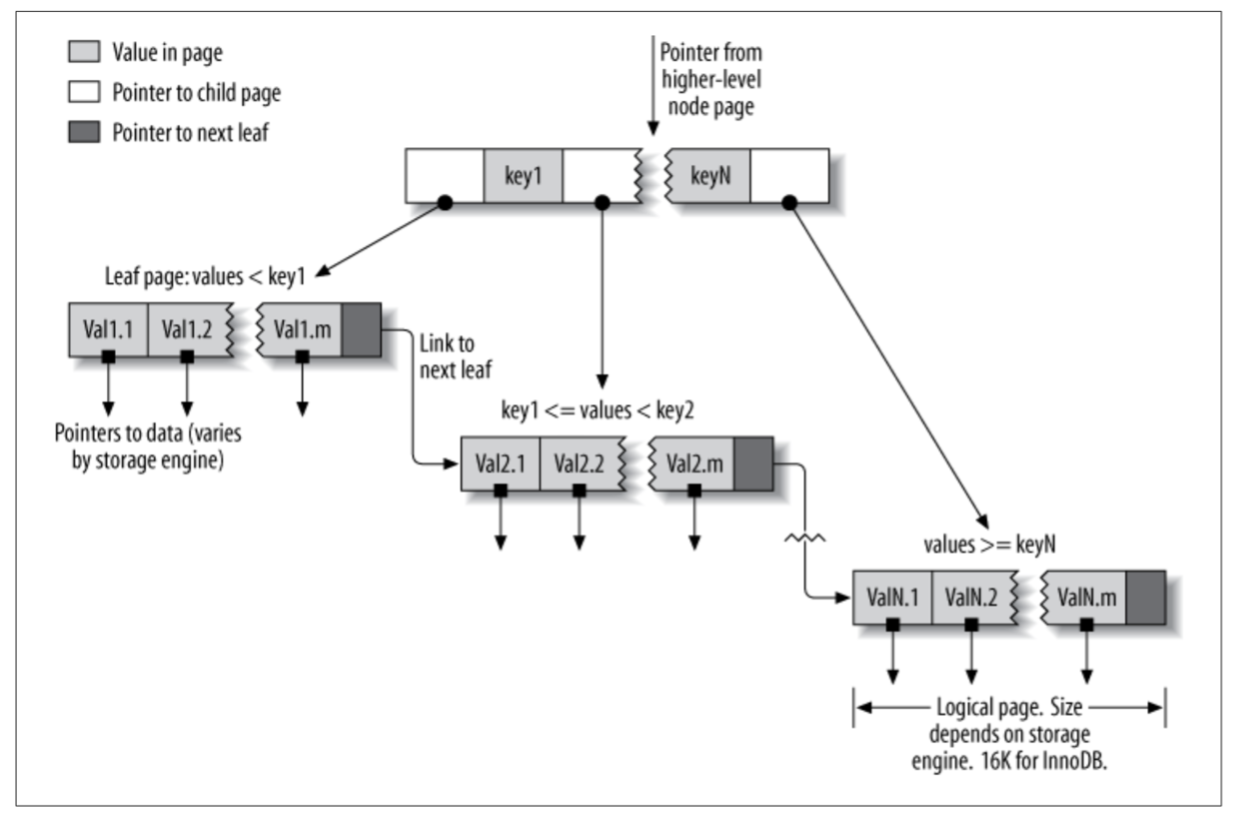
\includegraphics[width=0.65\textwidth]{PNGs/Textbook/B_Tree_Visualisation}
    \caption[Binärbaum-Visualisierung]{Binär-Baums-Darstellung (Abbildung 5--1 aus \cite[S. 149]{schwartz2012high})}
    \label{fig:b-tree-visualisation}
\end{figure}
\vspace{-20pt}

Die Blätter sind besonders, da sie Zeiger auf die indexierten Daten enthalten, anstatt auf andere Seiten zu verweisen.
Zwischen dem Wurzelknoten und den Blattseiten können viele Ebenen von Knoten-Seiten existieren.
Die Tiefe des Baumes hängt von der Größe der Tabelle ab.
Außerdem speichern B-Bäume die indexierten Spalten in einer festgelegten Reihenfolge, was sie besonders nützlich für die Suche nach Datenbereichen macht.
Beispielsweise kann ein Index auf einem Textfeld (z.B.\ vom Typ \texttt{VARCHAR}) effizient alle Namen finden, die mit „K“ beginnen, da die Werte in alphabetischer Reihenfolge gespeichert sind.

Der Index sortiert die Werte entsprechend der Reihenfolge der in der \texttt{CREATE INDEX}-Anweisung angegebenen Spalten, beispielsweise kann man wie folgt ein Index erstellen:

\vspace{-5pt}
\begin{lstlisting}[language=SQL,caption=B-Baum-Index bestehend aus mehreren Attributen,label={lst:indexing-create-combined}]
CREATE INDEX combined_index ON KUNDEN(NAME, VORNAME, GEBURTSTAG);
\end{lstlisting}
\vspace{-8pt}

Als Nächstes werden die möglichen Abfragen betrachtet, bei denen B-Baum-Indizes besonders hilfreich sind, um ein besseres Verständnis für ihre optimale Nutzung zu gewinnen.
Eine Übereinstimmung mit dem vollständigen Schlüsselwert liefert Werte für alle Spalten im Index.
Eine beispielhafte Abfrage zur Suche nach allen Einträgen mit dem Index aus~\ref{lst:indexing-create-combined} ist die Suche nach allen Kunden, die Max Mustermann heißen und am 01.01.2000 geboren wurden.
Auch Abfragen, die nur mit dem linken Präfix übereinstimmen, können von diesem Index profitieren.
So lässt sich etwa gezielt nach dem Nachnamen „Mustermann“ suchen.
Ebenso ist es möglich, nur ein Spaltenpräfix zu verwenden, etwa um alle Nachnamen zu finden, die mit „M“ beginnen.
Ein weiterer Vorteil ergibt sich bei Bereichsabfragen, denn der Index kann effizient genutzt werden, um Nachnamen zwischen „Mustermann“ und „Müller“ zu ermitteln.
Darüber hinaus unterstützt ein B-Baum-Index auch Kombinationen aus exakten und Bereichsabfragen, beispielsweise wenn nach dem Nachnamen „Mustermann“ gesucht wird, während der Vorname innerhalb eines Bereichs liegt, etwa ab „Ma“.
Ein weiterer Vorteil von B-Baum-Indizes ist, dass sie aufgrund der sortierten Baumstruktur nicht nur Abfragen, sondern auch \texttt{ORDER BY}-Bedingungen effizient unterstützen können.

Es gibt jedoch Einschränkungen von B-Baum-Indizes, die dazu führen, dass andere Indextypen für bestimmte Szenarien besser geeignet sind.
Eine Einschränkung ist, dass die Suche nicht am rechten Ende des Indexes beginnen kann.
Beispielsweise ist der Beispiels-Index nicht dazu geeignet, alle Personen zu finden, die vor dem Jahr 2000 geboren wurden, ohne dass der Nachname und Vorname ebenfalls spezifiziert werden.
Für optimale Leistung kann es auch erforderlich sein, dass Indizes mit den gleichen Spalten, jedoch in unterschiedlicher Reihenfolge erstellt werden.
Auf diese Weise könnten mehr Kombinationen abgedeckt und zusätzlich einige Abfragen optimiert werden.

Im nächsten Abschnitt werden die Benchmarks durchgeführt, um das Verständnis für die Funktionsweise des B-Baum-Index zu bestätigen.
Dazu wird zunächst wieder die Kundentabelle (\ref{lst:tools-create-table-kunde}) erstellt und für den ersten Vergleich werden folgende Indizes definiert:

\vspace{-5pt}
\begin{lstlisting}[language=SQL,caption=Definition mehrere Indizes,label={lst:indexing-create-multiple}]
CREATE INDEX idx_stadt ON KUNDEN(STADT);
CREATE INDEX idx_postleitzahl ON KUNDEN(POSTLEITZAHL);
CREATE INDEX idx_geburtstag ON KUNDEN(GEBURTSTAG);
\end{lstlisting}
\vspace{-5pt}

Um die Effizienz dieser Indizes einordnen zu können, wird diese Konfiguration mit einer verglichen, bei der nur die Kundentabelle ohne Indizes erstellt wird.
In beiden Fälle werden eine bestimmte Anzahl an Datensätze eingefügt.
Um die Performance der Select-Abfragen zu messen, werden verschiedene Queries an die Datenbank ausgeführt, bei denen die Attribute \texttt{GEBURTSTAG}, \texttt{STADT} und \texttt{POSTLEITZAHL} berücksichtigt werden.
Dazu gehören \texttt{GROUP BY}- und \texttt{COUNT}-Abfragen, bei denen die Index-Attribute verwendet werden oder sie spielen in der \texttt{WHERE}-Bedingung eine Rolle.
Damit es übersichtlich bleibt, werden einmal 10 Datensätze mit 40 und einmal 400 mit 4000 Zeilen verglichen.

\begin{figure}[H]
    \centering
    \begin{subfigure}[t]{0.48\textwidth}
        \centering
        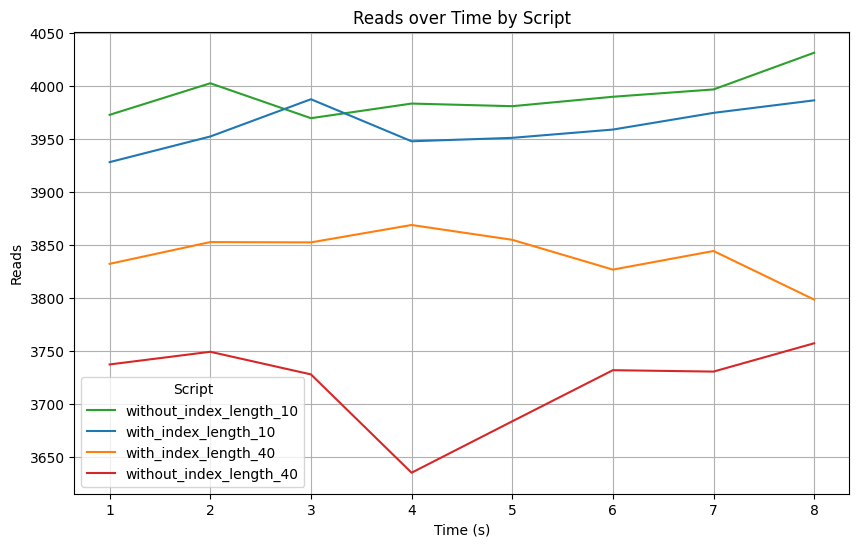
\includegraphics[width=\textwidth]{PNGs/Script/Index/B_Tree/low-count/Reads}
        \caption{Mit 10 und 40 Datensätze}
        \label{indexing-b-tree-low-reads}
    \end{subfigure}
    \hfill
    \begin{subfigure}[t]{0.48\textwidth}
        \centering
        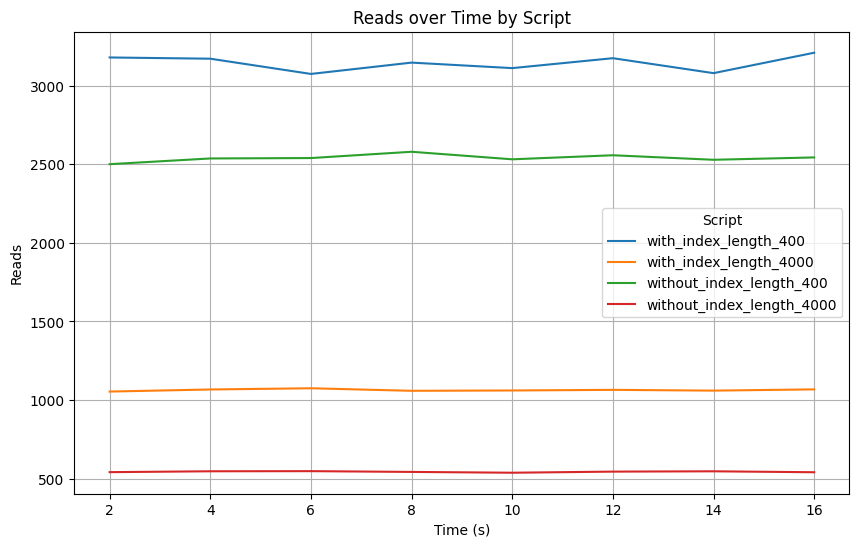
\includegraphics[width=\textwidth]{PNGs/Script/Index/B_Tree/high-count/Reads}
        \caption{Mit 400 und 4000 Zeilen}
        \label{indexing-b-tree-high-reads}
    \end{subfigure}
    \caption[B-Tree-Indexing: Mit Index vs Ohne]{Grafik zeigt Performance mit und ohne Index für Readsabfragen}
    \label{fig:indexing-vs-no}
\end{figure}
\vspace{-15pt}

In der Abbildung~\ref{indexing-b-tree-low-reads} ist zu erkennen, dass bei 10 Datensätzen die Kundentabelle ohne Indizes schneller ist als die mit Indizes.
Bei 40, 400 oder 4000 Zeilen (siehe~\ref{indexing-b-tree-high-reads}) wird schon die Wirkung der Indizes deutlich, da in diesen Fällen jeweils die Version mit Indizes effizienter ist.
Der Unterschied bei 40 Datensätzen ist zwar etwas geringer, aber in den anderen Fällen sehen noch eindeutigere Unterschiede.
Interessant ist, dass es nicht linear oder quadratisch mit der Anzahl an Datensätzen in der Tabelle steigt, sondern bei 400 und 4000 Zeilen beträgt der Unterschied zur Tabelle ohne Index jeweils etwa 500--700 Abfragen.
Bei der Schreibgeschwindigkeit liegen beide auf einem sehr ähnlichen Niveau, wobei die Version ohne Index tendenziell einen leichten Vorteil hat.

Mit dem vorherigen Benchmark können die Vorteile eines Indexes bereits deutlich erkannt werden.
Nun soll jedoch auch die Funktionalität des B-Tree-Indexes in Bezug auf unterschiedliche Selects untersucht werden.
Dazu wird erneut die Kundentabelle erstellt, aber diesmal wird nur ein Index definiert (siehe~\ref{lst:indexing-create-combined}).

Anschließend wird die Tabelle mit einer festgelegten Anzahl an Datensätzen befüllt und es werden unterschiedliche Select-Befehle ausgeführt.
Im Codeblock~\ref{lst:indexing-b-tree-selects} sind aus Platzgründen nur die Where-Bedingungen zu sehen und am Ende jeder Zeile steht der Name der Query, damit später in der Analyse nachvollzogen werden kann, welche Query welche Performance liefert.

\newpage
\begin{lstlisting}[language=SQL,caption=Unterschiedliche Where-Bedingungen für B-Tree-Index,label={lst:indexing-b-tree-selects},basicstyle=\ttfamily\scriptsize]
WHERE NAME LIKE 'M%'; -- columm_prefix
WHERE NAME = 'Müller' AND VORNAME = 'Max' AND GEBURTSTAG < '1980-01-01'; -- combined_match_with_range
WHERE NAME = 'Müller' AND VORNAME LIKE 'M%' ORDER BY GEBURTSTAG; -- exact_with_prefix
WHERE NAME = 'Müller' AND VORNAME = 'Max' AND GEBURTSTAG = '1960-01-01'; -- full_match
WHERE NAME = 'Müller'; -- leftmost_prefix
WHERE GEBURTSTAG < '1980-01-01'; -- not_leftmost
WHERE NAME BETWEEN 'Müller' AND 'Schulz'; -- range_values
WHERE NAME = 'Müller' AND VORNAME LIKE 'M%' AND GEBURTSTAG < '1980-01-01'; -- range_with_like
WHERE NAME = 'Müller' AND GEBURTSTAG < '1980-01-01'; -- skip_columns
\end{lstlisting}
\vspace{-5pt}

Anhand der Grafik in Abbildung~\ref{fig:indexing-b-tree-query-reads} lässt sich erkennen, bei welchen Abfragen der Index am effizientesten ist.
Auf der linken Seite können die Ergebnisse für die Read-Befehle mit Index betrachtet werden, während auf der rechten Seite die Werte ohne Index zu sehen sind.

\vspace{-5pt}
\begin{figure}[H]
    \centering
    \begin{subfigure}[t]{0.48\textwidth}
        \centering
        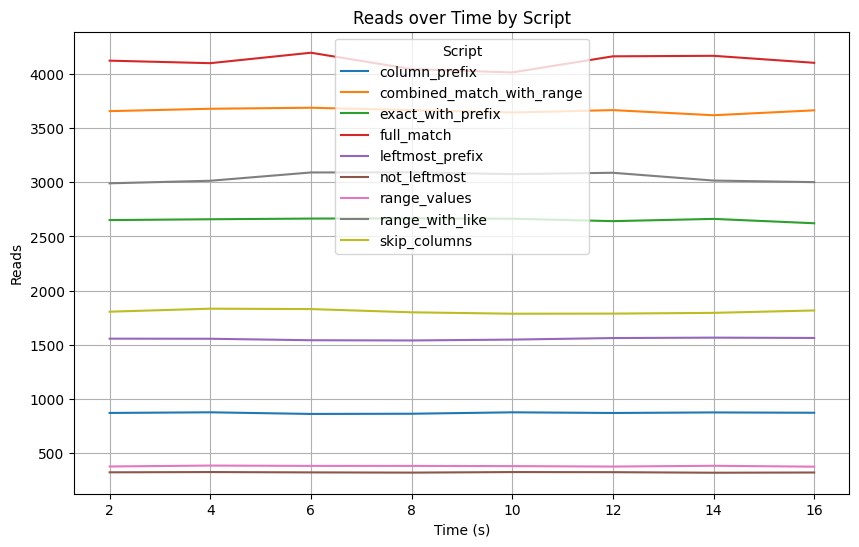
\includegraphics[width=\textwidth]{PNGs/Script/Index/B_Tree/b-tree-query-differences/Reads}
        \caption{Mit Index}
        \label{indexing-b-tree-query-reads-index}
    \end{subfigure}
    \hfill
    \begin{subfigure}[t]{0.48\textwidth}
        \centering
        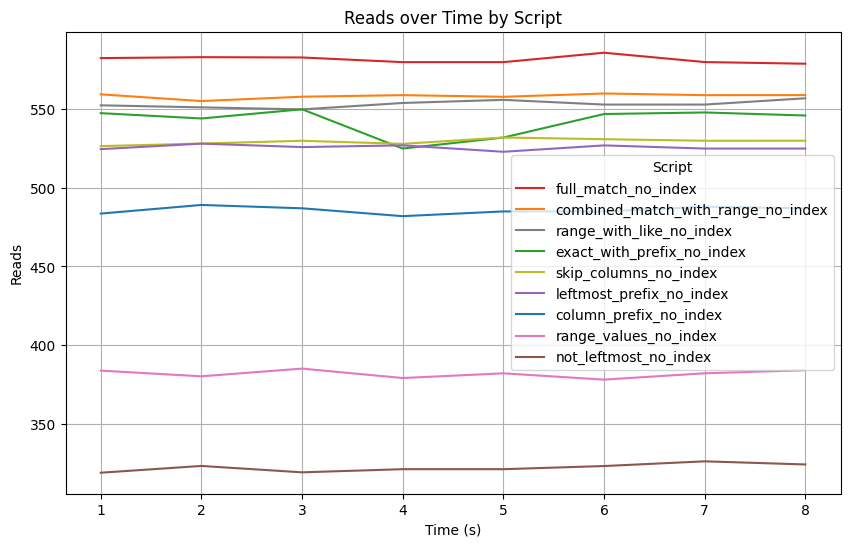
\includegraphics[width=\textwidth]{PNGs/Script/Index/B_Tree/b-tree-query-differences-no-index/Reads}
        \caption{Ohne Index}
        \label{indexing-b-tree-query-reads-no-index}
    \end{subfigure}
    \vspace{-5pt}
    \caption[B-Tree-Indexing: Unterschiedliche Selects mit Index und Ohne]{Visualisierung von unterschiedlichen Select-Queries mit und ohne Index}
    \label{fig:indexing-b-tree-query-reads}
\end{figure}
\vspace{-15pt}

Zunächst fällt auf, dass die Reihenfolge für die Werte mit und ohne Index komplett identisch ist.
Dies ist direkt erkennbar, da die Legenden beider Grafiken nach dem durchschnittlichen Wert über die gesamte Zeit sortiert sind.
Damit die richtigen Schlüsse aus der Grafik gezogen werden können, muss zunächst ermittelt werden, wie viele Zeilen die unterschiedlichen Queries zurückgeben.
Dazu werden die Abfragen zusätzlich mit dem \texttt{COUNT(*)}-Operator durchgeführt und die Ergebnisse in die Log-Datei geschrieben.
Anschließend werden die Werte entnommen und in einer Tabelle zusammengefasst.

\vspace{-5pt}
\begin{table}[H]
    \centering
    \scriptsize
    \begin{tabular}{|l|l|l|l|}
        \hline
        \textbf{Select-Query} & \textbf{Anzahl an Zeilen} & \textbf{Faktor} & \textbf{Index benutzt?} \\
        \hline
        full\_match & 0 & 6.42 & ja \\
        combined\_match\_with\_range & 13 & 5.78 & ja \\
        range\_with\_like & 31 & 5.22 & ja \\
        exact\_with\_prefix & 51 & 5.14 & ja \\
        skip\_columns & 147 & 3.47 & ja \\
        leftmost\_prefix & 263 & 2.73 & ja \\
        column\_prefix & 551 & 1.69 & ja \\
        range\_values & 1343 & 0.96 & nein \\
        not\_leftmost & 2371 & 0.98 & nein \\
        \hline
    \end{tabular}
    \vspace{3pt}
    \caption{Ergebnisse der COUNT(*)-Abfragen für B-Tree-Index}
    \label{tab:indexing_b_tree_count_results}
\end{table}
\vspace{-25pt}

Anhand der Spalte \texttt{Anzahl an Zeilen} lässt sich erkennen, dass die Queries, die am wenigsten Zeilen zurückgeben, auch diejenigen sind, bei denen die höchste Performance erzielt wird.
Deshalb ist auch die Reihenfolge mit und ohne Index gleich, weshalb man meinen könnte, dass der Index keinen Einfluss auf die Performance hat.
Dies betrifft jedoch nur die Reihenfolge, nicht aber die Werte der Abfragen, da hier deutliche Unterschiede erkennbar sind.
Anschaulich wird das mit der Betrachtung der Spalte \texttt{Faktor}.
Um den Wert zu berechnen, werden die Werte aus der Gesamtstatistik entnommen und die Version mit Index durch die Version ohne Index geteilt.
Dadurch lässt sich erkennen, dass \texttt{full\_match} zwar bei beiden Versionen am schnellsten ist, jedoch mit Index etwa 6-mal schneller als ohne.
Es lässt sich auch erkennen, dass je weniger Zeilen zurückgegeben werden, desto größer ist der Faktor.
Bei den Queries \texttt{range\_values} und \texttt{not\_leftmost} liegt der Faktor sehr nah 1, was bedeutet, dass der Index keinen Einfluss auf die Performance hat.
Deshalb stellt sich auch die Frage, ob der Index überhaupt verwendet wird.
Um das zu überprüfen, wird der \texttt{EXPLAIN}-Operator verwendet, das Ergebnis erneut geloggt und der Tabelle hinzugefügt (siehe Spalte \texttt{Index benutzt?}).
Und tatsächlich sehen wir, dass die vermuteten Queries die einzigen sind, bei denen der Index nicht verwendet wird.

\section{Hash-Index}\label{sec:indexing-hash-index}
Ein weiterer Indextyp, der betrachtet wird, ist der Hash-Index.
Dieser basiert auf einer Hash-Tabelle und ist daher nur für exakte Suchanfragen geeignet, die alle Spalten des Indexes verwenden.
In MySQL unterstützt nur die Memory-Storage-Engine explizite Hash-Indizes.
Einige Storage-Engines, wie zum Beispiel InnoDB, können erkennen, wenn bestimmte Index-Werte besonders häufig abgefragt werden.
Sie erstellen dann automatisch einen Hash-Index für diese Werte im Speicher, der zusätzlich zu den bestehenden B-Baum-Indizes genutzt wird.
Die Funktionsweise der Storage-Engine lässt sich wie folgt beschreiben.

Für jede Zeile wird mithilfe einer Hash-Funktion ein Hash-Wert der indexierten Spalte berechnet.
Der Hash-Wert (engl.\ hash code) ist eine kleine Zahl, die sich in der Regel von den Hash-Werten anderer Zeilen mit unterschiedlichen Schlüsselwerten unterscheidet.
Anschließend wird die Position im Index gesucht und man findet einen Zeiger auf die entsprechende Zeile.
In letzten Schritt überprüft man die Werte der Zeile, um sicherzustellen, dass es sich um die richtige Zeile handelt.

Wenn mehrere Werte denselben Hash-Wert besitzen, speichert der Index die Zeiger auf die Zeilen (engl.\ row pointers) in demselben Hash-Tabelleneintrag, typischerweise mithilfe einer verketteten Liste (z.B.\ einer \textit{Linked List}).
Hash-Kollisionen können die Leistung eines Hash-Index beeinträchtigen, da jeder Zeiger in der verketteten Liste durchlaufen und die entsprechenden Werte mit dem Suchwert verglichen werden müssen, um die richtigen Zeilen zu finden.
Das ist auch Index-Wartungsoperationen mit viel Aufwand verbunden.
Hingegen eindeutige Hash-Indizes stellen sicher, dass für jeden Hash-Wert nur ein einziger Eintrag existiert.
Bei Konflikten wird ein Mechanismus wie die Open Addressing-Strategie (z.B.\ Linear Probing oder Quadratic Probing) eingesetzt, um Konflikte zu lösen und den Speicherplatz effizient zu verwalten.
Hierbei wird versucht, Konflikte direkt innerhalb der Hash-Tabelle zu bewältigen, anstatt auf zusätzliche Datenstrukturen wie verkettete Listen zurückzugreifen.
Die eindeutigen Hash-Indizes werden nicht von der Memory-Engine in MySQL unterstützt.

Um die Verwendung des Hash-Indexes zu veranschaulichen, benutzen folgt folgendes Beispiel:

\vspace{-5pt}
\begin{lstlisting}[language=SQL]
SELECT * FROM KUNDEN WHERE NAME = 'Peter';
\end{lstlisting}
\vspace{-8pt}

Zunächst berechnet MySQL den Hash-Wert für \texttt{'Peter'} und verwendet diesen, um den entsprechenden Zeiger im Index zu finden.
Angenommen, die Hash-Funktion liefert für \texttt{'Peter'} den Wert \textbf{7654}.
MySQL sucht nun im Index an der Position 7654 und findet einen Zeiger auf Zeile 3.
Im letzten Schritt wird der Wert in Zeile 3 mit \texttt{'Peter'} verglichen.
Da die Indizes nur kompakte Hash-Werte speichern, sind Hash-Indizes äußerst platzsparend und Suchvorgänge erfolgen in hoher Geschwindigkeit.

Ähnlich wie der B-Baum-Index hat auch der Hash-Index einige Einschränkungen.
Zum einen enthält der Index nur Hash-Werte und Zeiger auf Zeilen (engl.\ row pointers), jedoch nicht die Werte selbst.
Deshalb kann MySQL den Index nicht verwenden, um das Einlesen der Zeilen zu vermeiden.
Allerdings erfolgt der Zugriff auf die in den Speicher geladenen Zeilen sehr schnell, wodurch die Leistung nicht wesentlich beeinträchtigt ist.
Zum anderen können Hash-Indizes nicht für Sortierungen verwendet werden, da die Werte nicht in einer geordneten Reihenfolge gespeichert sind.
Im Gegensatz dazu sind B-Baum-Indizes in der Lage.
Darüber hinaus ermöglichen Hash-Indizes keine partiellen Schlüsselübereinstimmungen (engl.\ partial key matching).
Da der Hash-Wert aus dem gesamten indexierten Wert berechnet wird, hilft ein Hash-Index beispielsweise nicht, wenn ein Index aus den Spalten (A, B) besteht und die \texttt{WHERE}-Klausel nur auf A verweist.
Ein weiterer Nachteil besteht darin, dass Hash-Indizes keine Bereichsabfragen unterstützen.
Sie eignen sich lediglich für Gleichheitsvergleiche, wie die Operatoren \texttt{=} (gleich), \texttt{<=>} (null-sicher gleich) und \texttt{IN()}.

Als Nächstes werden die Benchmarks mit Hash-Indizes betrachtet.
Dazu wird erneut die Kundentabelle verwendet und diesmal nur ein Index für die Spalte \texttt{NAME} erstellt.
Am Ende des \texttt{CREATE INDEX}-Befehls muss \texttt{USING HASH} hinzugefügt werden, damit statt des standardmäßigen B-Tree-Index der Hash-Index verwendet wird.
Danach befüllen wieder die Tabelle mit Testdaten.
Diesmal wird beim ersten Benchmark der Einfluss von Hash-Kollisionen auf die Performance untersucht.
Um den Grad der Kollisionen zu verändern, wird eine Variable verwendet, die die obere Grenze für die zufällige Generierung einer Zahl darstellt.
Anschließend werden alle Zeilen mit dem Wert \texttt{Kunde\_1} für die Spalte \texttt{NAME} abgefragt und die Tests werden mit den Kollisionswahrscheinlichkeiten von 25\%, 10\%, 5\% und 1\% durchgeführt.

\vspace{-4pt}
\begin{figure}[H]
    \centering
    \begin{subfigure}[t]{0.48\textwidth}
        \centering
        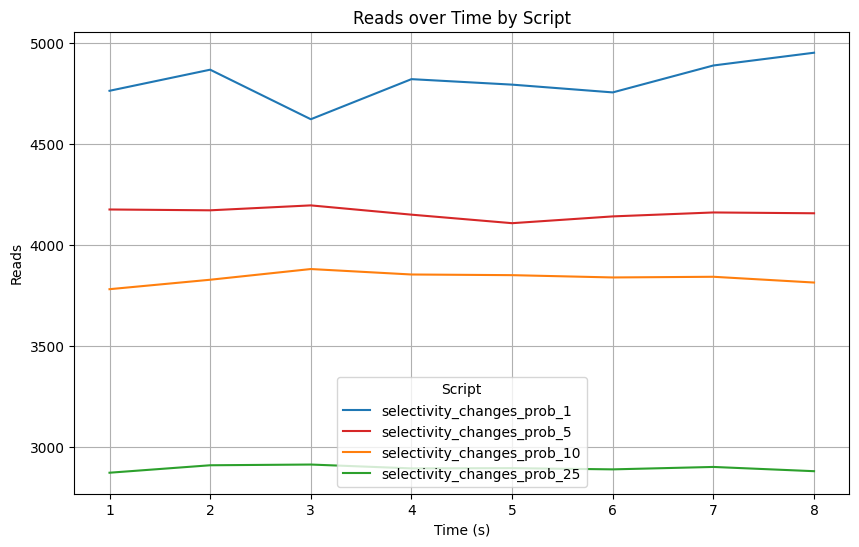
\includegraphics[width=\textwidth]{PNGs/Script/Index/Hash/hash-selectivity-change/Reads}
    \end{subfigure}
    \hfill
    \begin{subfigure}[t]{0.48\textwidth}
        \centering
        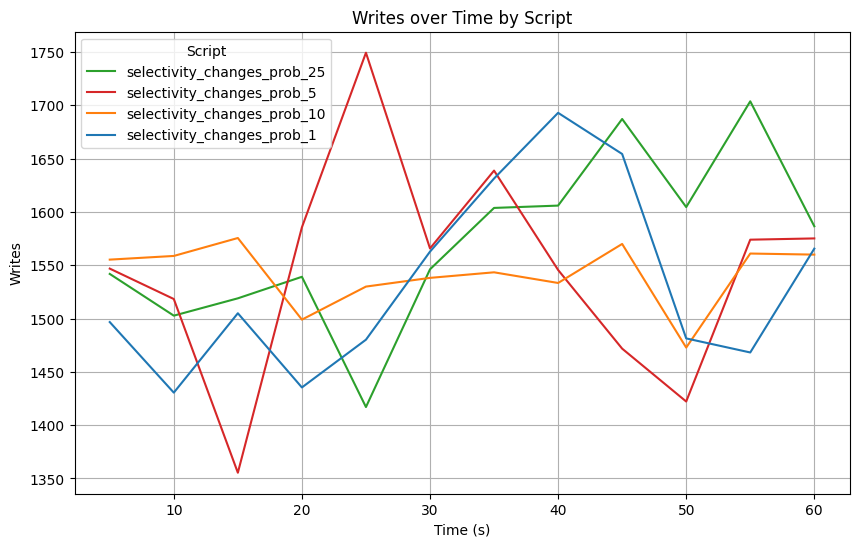
\includegraphics[width=\textwidth]{PNGs/Script/Index/Hash/hash-selectivity-change/Writes}
    \end{subfigure}
    \vspace{-8pt}
    \caption[Hash-Indexing: Auswirkungen von Hashkollisionen]{Vergleich der Auswirkungen von Hashkollisionen}
    \label{fig:hash-collision-comparison}
\end{figure}
\vspace{-17pt}

An den Ergebnissen in Abbildung~\ref{fig:hash-collision-comparison} ist zu erkennen, dass je geringer die Wahrscheinlichkeit für eine Kollision ist, desto schneller fällt die Select-Abfrage aus.
Es fällt auch auf, dass die Unterschiede zwischen den verschiedenen Kollisionswahrscheinlichkeiten sehr groß sind.
Hingegen die Einfüge-Performance ist bei allen 4 Varianten auf einem ähnlichen Niveau.

Als zweiten Test soll überprüft werden, ob der Index bei bestimmten Select-Queries benutzt wird oder nicht.
Dazu wird erneut die Kundentabelle verwendet, der gleiche Index wie in Beispiel~\ref{lst:indexing-create-combined} erstellt, die Testdaten eingefügt und die Select-Befehle aus~\ref{lst:indexing-b-tree-selects} genutzt.
Dieses Mal werden aber nicht alle Select-Befehle verwendet, sondern nur die aus folgender Tabelle:

\vspace{-4pt}
\begin{table}[H]
    \centering
    \scriptsize
    \begin{tabular}{|l|l|l|l|}
        \hline
        \textbf{Select-Query} & \textbf{Anzahl an Zeilen} & \textbf{Faktor} & \textbf{Index benutzt?} \\
        \hline
        full\_match & 0 & 2.67 & ja \\
        combined\_match\_with\_range & 6 & 0.97 & nein \\
        exact\_with\_prefix & 45 & 1.01 & nein \\
        leftmost\_prefix & 206 & 1.00 & nein \\
        \hline
    \end{tabular}
    \vspace{3pt}
    \caption{Ergebnisse der COUNT(*)-Abfragen für Hash-Index}
    \label{tab:indexing_hash_count_results}
\end{table}
\vspace{-30pt}

Anhand der Spalten \texttt{Faktor} und \texttt{Index benutzt?} kann erkannt werden, dass der Index nur bei der \texttt{full\_match}-Abfrage benutzt wird.
Das stimmt auch mit den Ergebnissen aus der Abbildung~\ref{fig:indexing-hash-query-reads} überein, da ohne Index alle Abfragen auch einem ähnlichen Niveau liegen, aber mit Index sticht eine deutlich hervor.
Interessant ist, dass die Query mit 206 zurückgegebenen Zeilen nur unwesentlich langsamer ist als die anderen.
Die Reihenfolge ist wieder bei beiden identisch und hängt von der Anzahl der zurückgegebenen Zeilen ab.

\vspace{-4pt}
\begin{figure}[H]
    \centering
    \begin{subfigure}[t]{0.48\textwidth}
        \centering
        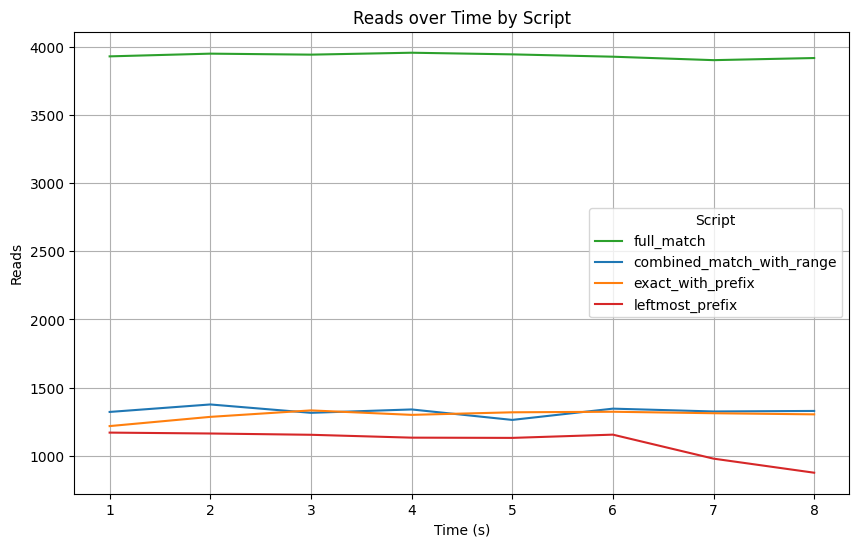
\includegraphics[width=\textwidth]{PNGs/Script/Index/Hash/hash-query-differences/Reads}
    \end{subfigure}
    \hfill
    \begin{subfigure}[t]{0.48\textwidth}
        \centering
        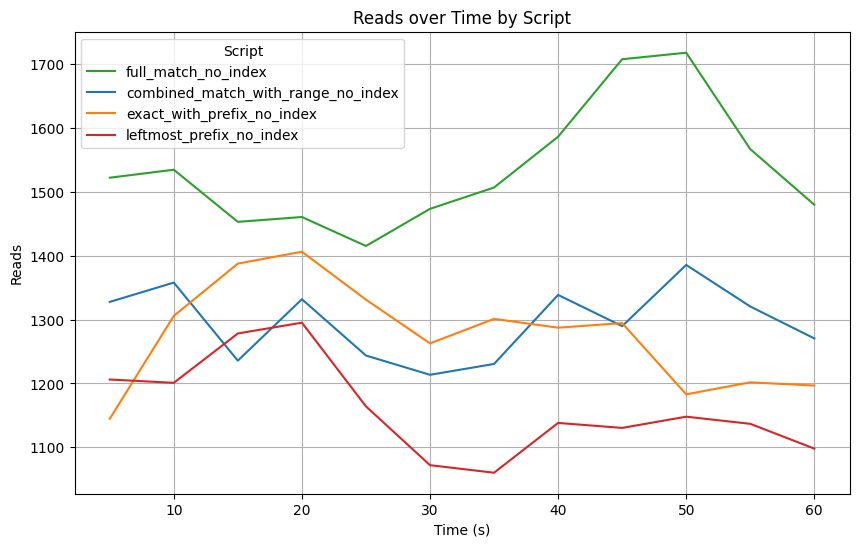
\includegraphics[width=\textwidth]{PNGs/Script/Index/Hash/hash-query-differences-no-index/Reads}
    \end{subfigure}
    \vspace{-8pt}
    \caption[Hash-Indexing: Unterschiedliche Abfragen mit Index und Ohne]{Grafik visualisiert Select-Queries mit (links) und ohne (rechts) Index}
    \label{fig:indexing-hash-query-reads}
\end{figure}

\section{Vergleich von B-Tree- und Hash-Index}\label{sec:indexing-comp-b-tree-hash-index}

In den vorherigen Kapiteln wurden der B-Tree-Index und der Hash-Index jeweils getrennt voneinander betrachtet.
Dabei wurde auch analysiert, bei welchen Select-Queries die Indizes Vorteile bieten und bei welchen nicht.
Damit fehlt uns noch der Vergleich zwischen dem B-Tree-Index und dem Hash-Index.

Um die Unterschiede zwischen beiden Indexstrukturen genauer zu analysieren, wird ein neuer Benchmark durchgeführt, der die Skripte aus Kapitel~\ref{sec:indexing-b-baum-index} und~\ref{sec:indexing-hash-index} wiederverwendet.
Da der Hash-Index aber nur 4 unterschiedliche Select-Queries aufruft, sollen auch nur diese mit dem B-Tree-Index ausgeführt werden.
Dazu wird einfach der Parameter~\texttt{selects} beim Aufruf des Orchestrator-Skripts hinzugefügt und das Skript anschließend ausgeführt.

\vspace{-4pt}
\begin{figure}[H]
    \centering
    \begin{subfigure}[t]{0.48\textwidth}
        \centering
        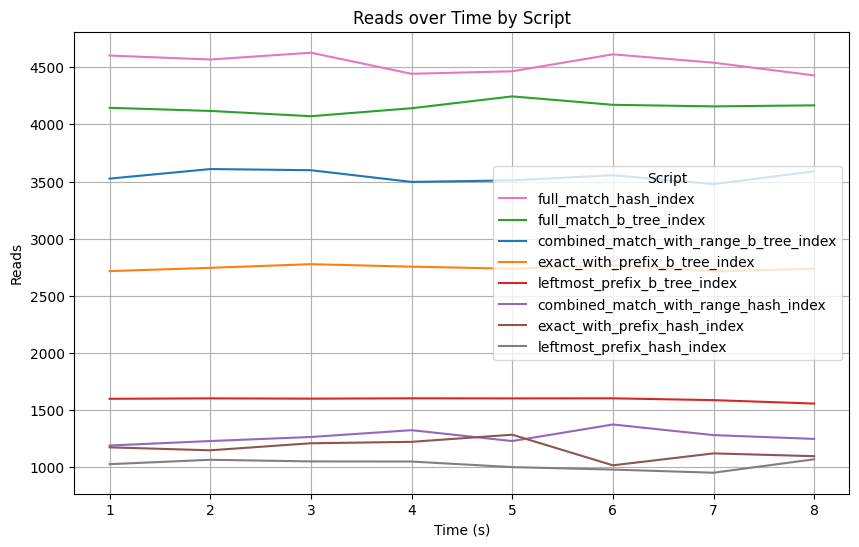
\includegraphics[width=\textwidth]{PNGs/Script/Index/B_Tree/hash-vs-b-tree-comparison/Reads}
        \caption{Anzahl der Lesezugriffe}
        \label{indexing-hash-vs-b-tree-comparison-reads}
    \end{subfigure}
    \hfill
    \begin{subfigure}[t]{0.48\textwidth}
        \centering
        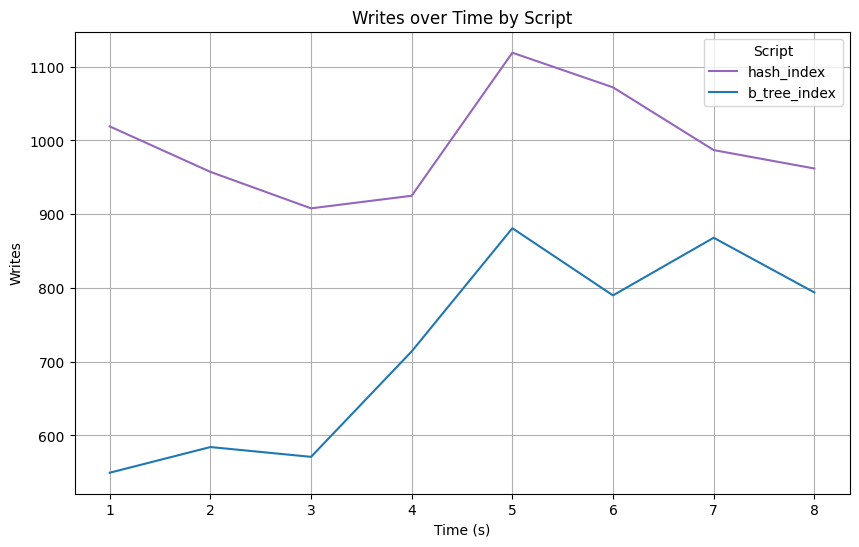
\includegraphics[width=\textwidth]{PNGs/Script/Index/B_Tree/hash-vs-b-tree-comparison/Writes}
        \caption{Anzahl der Schreibzugriffe}
        \label{indexing-hash-vs-b-tree-comparison-writes}
    \end{subfigure}
    \vspace{-2pt}
    \caption[Indexing: Vergleich von B-Tree- und Hash-Index]{Vergleich der Select-Query-Performance von B-Tree- und Hash-Index}
    \label{fig:indexing-hash-b-tree-comp}
\end{figure}
\vspace{-12pt}

In der Abbildung~\ref{indexing-hash-vs-b-tree-comparison-reads} sehen die Performance für die unterschiedlichen Select-Befehle.
Die höchste Transaktionsrate erzielt der Hash-Index, sofern der vollständige Schlüssel angegeben wird (\texttt{full\_match}).
Dicht darauf folgt der B-Tree-Index mit derselben Abfrage, allerdings mit etwa 10\% weniger Zugriffen.
Bei den übrigen Abfragen schneidet hingegen der B-Tree-Index deutlich besser ab, in einigen Fällen sogar bis zu dreimal schneller als der Hash-Index.
Der Grund dafür ist bereits aus den anderen Kapiteln bekannt.
Da der Hash-Index nur bei exaktem Schlüsselabgleich zum Einsatz kommt, wird er bei den anderen Abfragen nicht verwendet.
Mithilfe des \texttt{EXPLAIN}-Operators wurde festgestellt, dass stattdessen der B-Tree-Index verwendet wird, was die starken Unterschiede erklärt.

Betrachtet man die Schreibperformance (Abbildung~\ref{indexing-hash-vs-b-tree-comparison-writes}), zeigt sich, dass der Hash-Index etwa 30--40\% schneller ist als der B-Tree-Index.
Wenn eine Anwendung also eine hohe Schreiblast hat, könnte der Hash-Index eine bessere Wahl sein, da er weniger Mehraufwand verursacht.
Zusammenfassend lässt sich festhalten, dass der Hash-Index einen leichten Vorteil hat, wenn beide Indexe greifen.
Andernfalls überwiegen die Stärken des B-Tree-Indexes.

% -*- coding: utf-8 -*-

% Ausgabe des Literaturverzeichnisses; ohne weitere Optionen werden nur die
% Bücher und Artikel ausgegeben, die in der Arbeit auch zitiert werden.
\printbibliography

% markiert den Anfang des Anhangs
\appendix

% ein Kapitel, das nicht numeriert, aber trotzdem ins Inhaltsverzeichnis
% aufgenommen wird
\addchap{Anhang}
% TODO (Daniel): update here se-app
Hier beginnt der Anhang.  Siehe die Anmerkungen zur Sinnhaftigkeit eines
Anhangs in Abschnitt%~\ref{sec-app} auf Seite~\pageref{sec-app}.

Der Anhang kann wie das eigentliche Dokument in Kapitel und Abschnitte
unterteilt werden.  Der Befehl \verb|\appendix| sorgt im Wesentlichen nur für
eine andere Nummerierung.

% neue Seite
\clearpage

% keine Seitenzahl
\thispagestyle{empty}

% keine Nummerierung, keine Aufnahme ins Inhaltsverzeichnis
\section*{Eigenständigkeitserklärung}

% Hier müssen Sie natürlich den Titel der Arbeit sowie Ort und Datum ersetzen:
Hiermit versichere ich, dass ich die vorliegende Bachelorarbeit mit dem Titel
\begin{center}
  \textbf{Performance - Optimierung von Datenbanken}
\end{center}
selbstständig und nur mit den angegebenen Hilfsmitteln verfasst habe.  Alle
Passagen, die ich wörtlich aus der Literatur oder aus anderen Quellen wie
z.\,B. Internetseiten übernommen habe, habe ich deutlich als Zitat mit Angabe
der Quelle kenntlich gemacht.

\vspace{2cm}
% TODO (Daniel): update this here
Hamburg, 21.\ Dezember 1940

\end{document}